\section {Numerical Solution Technique}
\label{Num}

\subsection{Vertical and horizontal discretization}
\subsubsection{Horizontal grid}
\label{hori}
In the horizontal $(\xi,\eta)$, a traditional, centered, second-order
finite-difference approximation is adopted.  In particular, the
horizontal arrangement of variables is as shown in Fig.\ \ref{fcgr}.
This is equivalent to the well known Arakawa ``C'' grid, which is well
suited for problems with horizontal resolution that is fine compared to
the first radius of deformation (Arakawa and Lamb \cite{AL}).
\begin{figure}[htb]
\setlength{\unitlength}{6mm}
\thicklines
  \begin{picture}(19,12)(-8,0)
  \put(0,1.5){\line(1,0){12}}
  \put(0,8.5){\line(1,0){12}}
  \put(2,0){\line(0,1){10}}
  \put(10,0){\line(0,1){10}}
  \put(6,5){\circle{.4}}
\thinlines
  \put(6.5,9.6){\vector(1,0){3.5}}
  \put(5.5,9.6){\vector(-1,0){3.5}}
  \put(11.4,5.4){\vector(0,1){3.1}}
  \put(11.4,4.6){\vector(0,-1){3.1}}
  \put(1.5,5){\vector(1,0){1}}
  \put(9.5,5){\vector(1,0){1}}
  \put(6,1){\vector(0,1){1}}
  \put(6,8){\vector(0,1){1}}
  \put(6,9.6){\makebox(0,0){$\Delta\xi$}}
  \put(11.4,5){\makebox(0,0){$\Delta\eta$}}
  \put(6,5.4){\makebox(0,0)[b]{$(\rho,h,f,\Omega )_{i,j}$}}
  \put(1.8,5.3){\makebox(0,0)[br]{$u_{i,j}$}}
  \put(9.8,5.3){\makebox(0,0)[br]{$u_{i+1,j}$}}
  \put(5.8,1.3){\makebox(0,0)[tr]{$v_{i,j}$}}
  \put(5.8,8.3){\makebox(0,0)[tr]{$v_{i,j+1}$}}
  \end{picture}
\caption{Placement of variables on an Arakawa C grid}
\label{fcgr}
\end{figure}

\subsubsection{Vertical grid}
The vertical discretization also uses a second-order finite-difference
approximation.  Just as we use a staggered horizontal grid, the 
model was found to be more well-behaved with a staggered vertical
grid.  The vertical grid is shown in Fig.\ \ref{fvert}.

\begin{figure}[thb]
\setlength{\unitlength}{0.00083300in}%
%
\begin{picture}(987,2835)(-611,-3463)
\put(3166,-886){\circle*{120}}
\put(3166,-1336){\circle*{120}}
\put(3166,-1786){\circle*{120}}
\put(3166,-2236){\circle*{120}}
\put(3166,-2686){\circle*{120}}
\put(3166,-3136){\circle*{120}}
\put(2701,-661){\line( 1, 0){900}}
\put(3001,-1111){\line( 1, 0){300}}
\put(3001,-1561){\line( 1, 0){300}}
\put(3001,-2011){\line( 1, 0){300}}
\put(3001,-2461){\line( 1, 0){300}}
\put(3001,-2911){\line( 1, 0){300}}
\put(2701,-3361){\line( 1, 0){900}}
\put(3676,-736){\makebox(0,0)[lb]{$w_{\rm N}$}}
\put(3376,-961){\makebox(0,0)[lb]{$\rho_{\rm N}$}}
\put(3376,-3211){\makebox(0,0)[lb]{$\rho_1$}}
\put(3376,-2761){\makebox(0,0)[lb]{$\rho_2$}}
\put(3451,-2986){\makebox(0,0)[lb]{$w_1$}}
\put(3676,-3436){\makebox(0,0)[lb]{$w_0$}}
\put(3451,-2536){\makebox(0,0)[lb]{$w_2$}}
\put(3451,-1186){\makebox(0,0)[lb]{$w_{\rm N-1}$}}
\put(3376,-1411){\makebox(0,0)[lb]{$\rho_{\rm N-1}$}}
\end{picture}
\caption{Placement of variables on staggered vertical grid}
\label{fvert}
\end{figure}

\subsection{Masking of land areas}
\label{Mask1}
ROMS has the ability to work with interior land areas, although the
computations occur over the entire model domain.  One grid cell is
shown in Fig.\ \ref{fcgr} while several cells are shown in Fig.\
\ref{fmask1}, including two land cells.  The process of defining which
areas are to be masked is external to ROMS and is usually
accomplished in \code{Matlab}; this
section describes how the masking affects the computation of the
various terms in the equations of motion.
\begin{figure}[t]
\setlength{\unitlength}{0.0125in}%
\begin{picture}(0,0)(-61,0)%
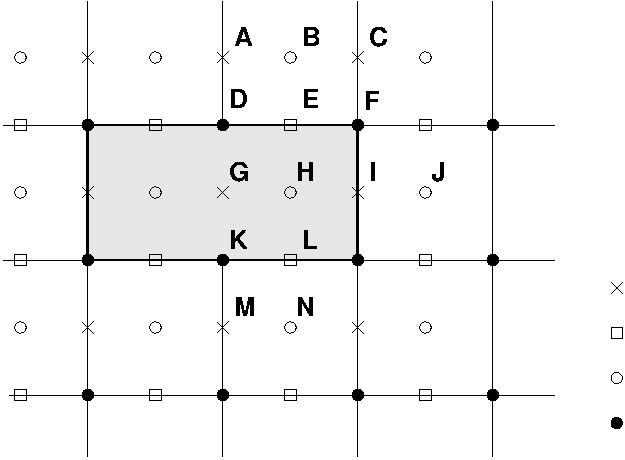
\includegraphics{pics/mask2}%
\end{picture}%
\begin{picture}(348,263)(92,465)
\put(490,552){\makebox(0,0)[lb]{-- $u$ points}}
\put(490,528){\makebox(0,0)[lb]{-- $v$ points}}
\put(490,504){\makebox(0,0)[lb]{-- $\rho$ points}}
\put(490,480){\makebox(0,0)[lb]{-- $\psi$ points}}
\end{picture}
\caption{Masked region within the domain}
\label{fmask1}
\end{figure}

\subsubsection{Velocity}
At the end of every time step, the values of many variables within the
masked region are set to zero by multiplying by the mask for either the
$u$, $v$ or $\rho$ points.  This is appropriate for the $v$ points {\bf
E} and {\bf L} in Fig.\ \ref{fmask1}, since the flow in and out of the
land should be zero.  It is likewise appropriate for the $u$ point at
{\bf I}, but is not necessarily correct for point {\bf G}.  The only
term in the $u$ equation that requires the $u$ value at point {\bf G}
is the horizontal viscosity, which has a term of the form
$\frac{\partial}{\partial \eta} \nu \frac{\partial u}{\partial \eta}$.
Since point {\bf G} is used in this term by both points {\bf A} and
{\bf M}, it is not sufficient to replace its value with that of the
image point for {\bf A}.  Instead, the term $\frac{\partial u}{\partial
\eta}$ is computed and the values at points {\bf D} and {\bf K} are
replaced with the values appropriate for either free-slip or no-slip
boundary conditions.  Likewise, the term $\frac{\partial}{\partial \xi}
\nu \frac{\partial v}{\partial \xi}$ in the $v$ equation must be corrected
at the mask boundaries.

This is accomplished by having a fourth mask array defined at the $\psi$
points, in which the values are set to be no-slip in \code{metrics}.
For no-slip boundaries, we count on the values inside
the land (point {\bf G}) having been zeroed out.  For point {\bf D}, the
image point at {\bf G} should contain minus the value of $u$ at point
{\bf A}.  The desired value of $\frac{\partial u}{\partial \eta}$ is
therefore $2 u_{\bf A}$ while instead we have simply $u_{\bf A}$.
In order to achieve the correct result, we multiply by a mask which
contains the value 2 at point {\bf D}.  It also contains a 2 at point
{\bf K} so that $\frac{\partial u}{\partial \eta}$ there will acquire
the desired value of $-2 u_{\bf M}$. The corner point {\bf F} is set to
have a value of 1.

\subsubsection{Temperature, salinity and surface elevation}

The handling of masks by the temperature, salinity and surface
elevation equations is similar to that in the momentum equations, and
is in fact simpler.  Values of $T$, $S$ and $\zeta$ inside the land
masks, such as point {\bf H} in Fig.\ \ref{fmask1}, are set to zero
after every time step.  This point would be used by the horizontal
diffusion term for points {\bf B}, {\bf J}, and {\bf N}.  This is
corrected by setting the first derivative terms at points {\bf E}, {\bf
I}, and {\bf L} to zero, to be consistent with a no-flux boundary
condition.
Note that the equation of state must be able to handle $T = S = 0$
since this is the value inside masked regions.

%\subsubsection{Free surface and pressure gradients}

%The surface elevation inside the land mask is simply used for setting
%the total depth and therefore the location of the $s$-coordinate
%surfaces.

\subsubsection{Wetting and drying}

There is now an option to have wetting and drying in the model, in
which a cell can switch between being wet or being dry as the tides
come in and go out, for instance. Cells which are masked out as in
Fig.~\ref{fmask1} are never allowed to be wet, however.
\begin{itemize}
   \item In the case of wetting and drying, a critical depth, $D_{crit}$,
is supplied by the user.
   \item The total water depth ($D=h+\zeta$) is compared to $D_{crit}$.
If the water level is less than this depth, no flux is allowed out
of that cell. Water can always flow in and resubmerge the cell.
  \item The wetting and drying only happens during the 2-D
computations; the 3-D computations see a depth of
$D_{crit}$ in the ``dry'' areas.
  \item The ice component now checks for dry cells when computing
the ice rheology.
\end{itemize}

\subsection{Time-stepping overview}

While time stepping the model, we have a stored history of the model fields
at time $n-1$, an estimate of the fields at the current time $n$, and
we need to come up with an estimate for time $n+1$. For reasons of
efficiency, we choose to use a split-explicit time step, integrating
the depth-integrated equations with a shorter time step than the full
3-D equations. There is an integer ratio $M$ between the time steps. The
exact details of how the time stepping is done vary from one version
of ROMS to the next, with the east coast ROMS described here being older
than other branches. Still, all versions have these steps:

\begin{enumerate}
  \item Take a predictor step for at least the 3-D tracers to time
  $n+\frac{1}{2}$.
  \item Compute $\overline{\rho}$ and
$\rho^*$ for use in the depth-integrated time steps, from the density
either at time $n$ or time $n+\frac{1}{2}$.
  \item Depth integrate the 3-D momentum right-hand side terms at
time $n+\frac{1}{2}$ for use in the depth-integrated time steps (or extrapolate
to obtain an estimate of those terms).
  \item Take all the depth-integrated steps. Store weighted
time-means of the $\overline{u}$, $\overline{v}$ fields centered at both
time $n+\frac{1}{2}$ and time $n+1$ (plus $\zeta$ at time $n+1$). The latter
requires this time stepping to extend past time $n+1$, using $M^*$ steps
rather than just $M$.
  \item Use the weighted time-means from depth-integrated fields to
complete the corrector step for the 3-D fields to time $n+1$.
\end{enumerate}
Great care is taken to avoid the introduction of a mode-splitting
instability due to the use of shorter time steps for the depth-integrated
computations.

The mode coupling has evolved through the various ROMS versions,
as shown in Fig.~\ref{ftimestep1} (from \cite{SS2008a}). The time stepping
schemes are also listed in Table~\ref{ttimestep1} and described in
detail in \cite{SS2005} and \cite{SS2008b}; the relevant ones
are described in Appendix~\ref{Frog}.

\begin{figure}[p]
\setlength{\unitlength}{1.0in}%
%
\begin{picture}(6.5,7.5)(0,0)
  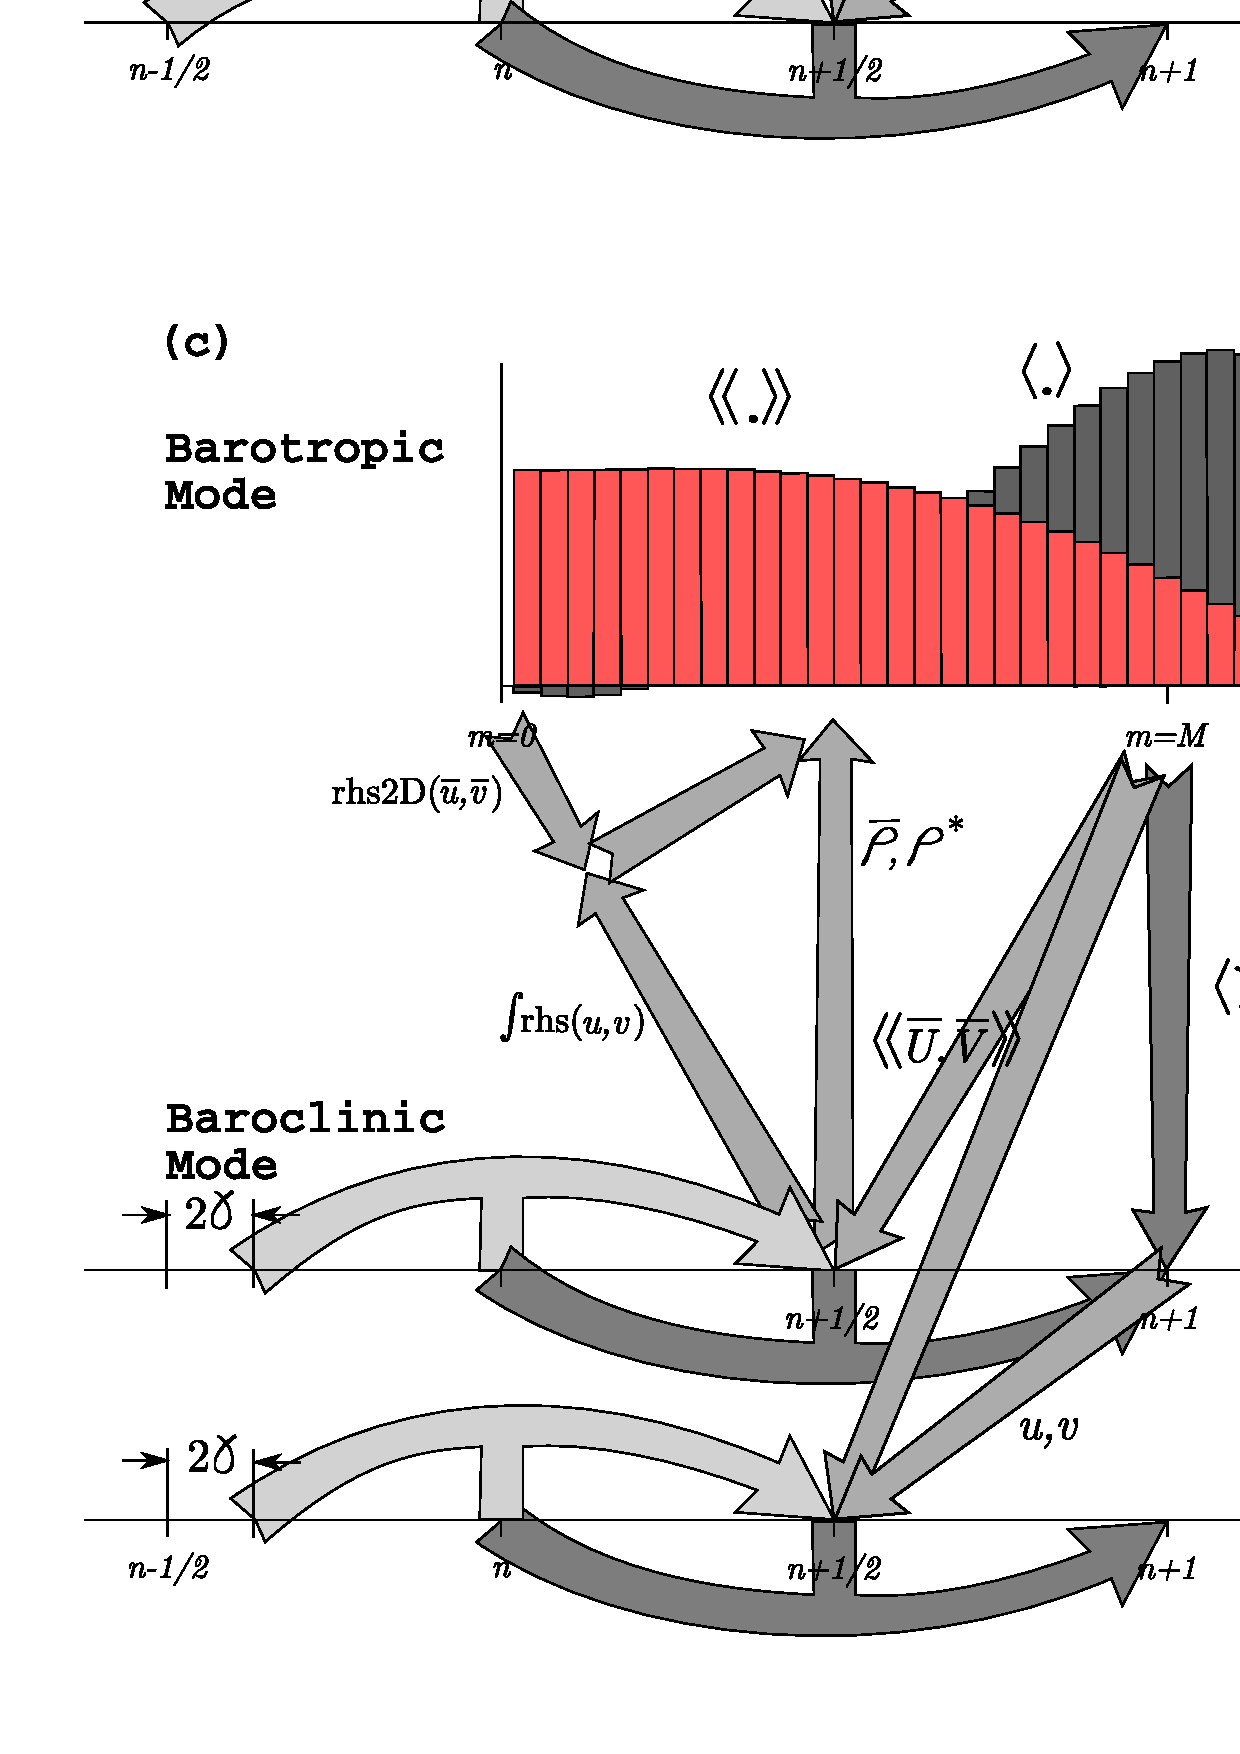
\includegraphics[width=6.5in]{pics/timestep_all}%
\end{picture}%
\caption{Diagrams of the time stepping and mode coupling used in
various ROMS versions. (a) Rutgers University ROMS (from
myroms.org), (b) ROMS AGRIF, (c) UCLA ROMS, described in \cite{SS2005},
(d) non-hydrostatic ROMS (\cite{Kanarska2007}). In all, the curved
arrows update the 3-D fields; those with ``pillars'' are leapfrog
in nature with the pillar representing the r.h.s. terms. Straight
arrows indicate exchange between the barotropic and baroclinic
modes. The shape functions for the fast time steps show just one
option out of many possibilities. The grey function has weights to
produce an estimate at time $n+1$, while the light red function has
weights to produce an estimate at time $n+\frac{1}{2}$.}
 \label{ftimestep1}
\end{figure}

\begin{table}[thb]
 \centerline{
\begin{tabular}{|l|c|c|c|c|c|} \hline
  & SCRUM 3.0 & Rutgers & AGRIF & UCLA & Non-hydrostatic \\
  \hline
  Reference & \cite{Hedstrom2000} & \cite{DAMEE_1} &
  \cite{Penven2006} & \cite{SS2005} & \cite{Kanarska2007} \\
  \hline
  Barotropic  & LF-TR & LF-AM3 with
  & LF-AM3 with & Gen. FB & Gen. FB \\
  mode & & FB feedback & FB feedback\footnote{The generalized FB
  barotropic mode was ported into the newest AGRIF code at the end
  of 2007.} & (AB3-AM4) & (AB3-AM4) \\
  \hline
  2-D $\alpha_{\max}$, iter. & $\sqrt{2}$,
  (2)\footnote{The number in parentheses (e.g., 2) indicates the
  number of r.h.s. computations per time step. If there are two
  parenthesized number, the first one is for momenta, the second for
  tracers.} & 1.85, (2) & 1.85,
  (2) & 1.78, (1) & 1.78, (1) \\
  \hline
  3-D momenta & AB3 & AB3 & LF-AM3 & LF-AM3 & AB3 (mod) \\
  \hline
  Tracers & AB3 & LF-TR & LF-AM3 & LF-AM3 & AB3 (mod) \\
  \hline
  Internal & AB3 & Gen.\ FB &
  LF-AM3, & LF-AM3, &
  Gen.\ FB \\
  waves & & (AB3-TR) & FB feedback & FB feedback & (AB3-AM4) \\
  \hline
  $\alpha_{\max}$, advect. & 0.72 & 0.72 & 1.587 &
  1.587 & 0.78 \\
  \hline
  $\alpha_{\max}$, Cor. & 0.72 & 0.72 & 1.587 &
  1.587 & 0.78 \\
  \hline
  $\alpha_{\max}$, int. w. & 0.72, (1) & 1.14,
  (1,2) & 1.85, (2) &
  1.85, (2) & 1.78, (1) \\
  \hline
  \end{tabular}
  }
\label{ttimestep1}
\caption{The time stepping schemes used in the various ROMS versions.
$\alpha \equiv \omega \delta t$ is the Courant number and $\omega=ck$
is the frequency for a wave component with wavenumber $k$.}
\end{table}

\subsection{Conservation properties}
\label{Enrg}
From Shchepetkin and McWilliams (2005) \cite{SS2005}, we have a
tracer concentration equation in advective form:
\begin{equation}
  \frac{\partial C}{\partial t} + (u \cdot \nabla) C = 0
  \label{eqt1}
\end{equation}
and also a tracer concentration equation in conservation form:
\begin{equation}
   \frac{\partial C}{\partial t} + \nabla \cdot (u C) = 0.
  \label{eqt2}
\end{equation}
The continuity equation:
\begin{equation}
   ( \nabla \cdot u) = 0
\end{equation}
can be used to get from one tracer equation to the other.
As a consequence of eq.~(\ref{eqt1}), if the tracer is spatially
uniform, it will remain so regardless of the velocity field
(constancy preservation). On the other hand, as a consequence of
(\ref{eqt2}), the volume integral of the tracer concentration is conserved
in the absence of internal sources and fluxes through the boundary. Both
properties are valuable and should be retained when constructing numerical
ocean models.

The semi-discrete form of the tracer equation
(\ref{st15}) is:
\begin{equation}
   \frac{\partial}{\partial t} \left( \frac{H_z C}{m n} \right)
   + \delta_{\xi} \left(
   \frac{u \overline{H_z}^\xi \overline{C}^\xi }{\overline{n}^\xi} \right)
   + \delta_{\eta} \left(
   \frac{v \overline{H_z}^\eta \overline{C}^\eta }{\overline{m}^\eta} \right)
   + \delta_\sigma \left( \overline{C}^\sigma
   \frac{H_z \Omega}{m n} \right) =
\\ \vspace{2mm}
   \frac{ 1}{mn} \frac{\partial}{\partial \sigma}
   \left( \frac{K_m}{\Delta z} \frac{\partial C}{\partial \sigma} \right) +
   {\cal D}_C + {\cal F}_C
\label{tfull}
\end{equation}
Here $\delta_{\xi}$, $\delta_{\eta}$ and $\delta_\sigma$ denote simple
centered finite-difference approximations to $\partial / \partial \xi$,
$\partial / \partial \eta$ and $\partial / \partial \sigma$ with the
differences taken over the distances $\Delta\xi$, $\Delta\eta$ and
$\Delta \sigma$, respectively. $\Delta z$ is the vertical distance from one
$\rho$ point to another. $\overline{ ( \hspace{5mm} )}^{\xi}$,
$\overline{ ( \hspace{5mm} )}^{\eta}$ and $\overline{ ( \hspace{5mm}
)}^\sigma$ represent averages taken over the distances $\Delta\xi$, $\Delta
\eta$ and $\Delta \sigma$. % $I_\sigma^0$ indicates a second-order vertical
%integral computed as a sum from level $\sigma$ to the surface at
%$\sigma=0$.

The finite volume version of the same equation is no different,
except that a quantity $C$ is defined as the volume-averaged
concentration over the grid box $\Delta V$:
\begin{equation}
   C = \frac{mn}{H_z} \int_{\Delta V} \frac{H_z C}{mn} \delta \xi
   \, \delta \eta \, \delta \sigma
\end{equation}
The quantity  $\left(
\frac{u \overline{H_z}^\xi \overline{C}^\xi}{\overline{n}^\xi} \right)$
is the flux through an interface between adjacent grid boxes.

This method of averaging was chosen because it internally conserves
first moments in the model domain, although it is still possible to
exchange mass and energy through the open boundaries. The method is
similar to that used in Arakawa and Lamb \cite{AL}; though their
scheme also conserves enstrophy. Instead, we will focus on (nearly) retaining
constancy preservation while coupling the barotropic
(depth-integrated) equations and the baroclinic equations.

The time step in eq.~(\ref{tfull}) is assumed to be from time $n$ to
time $n+1$, with the other terms being evaluated at time
$n+\frac{1}{2}$ for second-order accuracy.
Setting $C$ to 1 everywhere reduces eq.~(\ref{tfull}) to:
\begin{equation}
   \frac{\partial}{\partial t} \left( \frac{H_z}{m n} \right)
   + \delta_{\xi} \left(
   \frac{u \overline{H_z}^\xi }{\overline{n}^\xi} \right)
   + \delta_{\eta} \left(
   \frac{v \overline{H_z}^\eta}{\overline{m}^\eta} \right)
   + \delta_\sigma \left( 
   \frac{H_z \Omega}{m n} \right) = 0
\label{contfull}
\end{equation}
If this equation holds true for the step from time $n$ to time $n+1$, then
our constancy preservation will hold.

In a hydrostatic model such as ROMS, the discrete continuity
equation is needed to compute vertical velocity rather than grid-box
volume $\frac{H_z}{m n}$ (the latter is controlled by changes in
$\zeta$ in the barotropic mode computations). Here, $\frac{H_z
\Omega}{m n}$ is the finite-volume flux across the {\em moving}
grid-box interface, vertically on the $w$ grid.

The vertical integral of the continuity eq.~(\ref{st17}), using
the vertical boundary conditions on $\Omega$, is:
\begin{equation}
   \frac{\partial}{\partial t} \left( \frac{\zeta}{mn} \right) +
   \delta_{\xi} \left(
   \frac{\overline{u} \overline{D}^\xi }{\overline{n}^\xi} \right)
   + \delta_{\eta} \left(
   \frac{\overline{v} \overline{D}^\eta}{\overline{m}^\eta} \right)
   = 0
\label{zeta1}
\end{equation}
where $\zeta$ is the surface elevation, $D= h+\zeta$ is the total
depth, and $\overline{u},\overline{v}$ are the depth-integrated
horizontal velocities. This equation and the corresponding 2-D
momentum equations are time stepped on a shorter time step than 
eq.~(\ref{tfull}) and the other 3-D equations. Due to the details in
the mode coupling, it is only possible to maintain constancy
preservation to the accuracy of the barotropic time steps.

\subsection{Depth-integrated equations}
\label{Vort}
The depth average of a quantity $A$ is given by:
\begin{equation}
   \overline{A} = \frac{1}{D} \int_{-1}^0 H_z A d\sigma
\end{equation}
where the overbar indicates a vertically averaged quantity and
\begin{equation}
   D \equiv \zeta(\xi, \eta, t) + h(\xi, \eta)
\end{equation}
is the total depth of the water column.  The vertical integral of
equation (\ref{st13}) is:
%{\samepage
\begin{multline}
   \frac{\partial}{\partial t} \left( \frac{D \overline{u}}{mn} \right)
   + \frac 
   {\partial}{\partial \xi} \left( \frac{D \overline{uu}}{n} \right )
   + \frac 
   {\partial}{\partial \eta} \left( \frac{D \overline{uv}}{m} \right)
   - \frac{Df\overline{v}}{mn}
\\ \vspace{1mm}
   - \left[ \overline{vv}
   \frac{\partial}{\partial \xi}
   \left( \frac{1}{n} \right) - \overline{uv}
   \frac{\partial}{\partial \eta} \left(
   \frac{1}{m} \right) \right] D = 
   - \frac{D}{n}
   \left( \frac{\partial \overline{\phi_2}}{\partial \xi} +
   g \frac{\partial \zeta}{\partial \xi} \right)
\\ \vspace{1mm}
   + \frac{ D}{mn}
   \left( \overline{\cal F}_u + \overline{\cal D}_{h_u} \right) 
   + \frac{1}{mn} \left( \tau^{\xi}_s - \tau^{\xi}_b \right)
\label{ubar1}
\end{multline}
%}
where $\phi_2$ includes the $\frac{\partial z}{\partial \xi}$ term,
$\overline{\cal D}_{h_u}$ is the horizontal viscosity, and the
vertical viscosity only contributes through the upper and lower
boundary conditions.  The corresponding vertical integral of equation
(\ref{st14}) is:
%{\samepage
\begin{multline}
   \frac{\partial}{\partial t} \left( \frac{D \overline{v}}{mn} \right)
   + \frac 
   {\partial}{\partial \xi} \left( \frac{D \overline{uv}}{n} \right )
   + \frac 
   {\partial}{\partial \eta} \left( \frac{D \overline{vv}}{m} \right)
   + \frac{Df\overline{u}}{mn}
\\ \vspace{1mm}
   + \left[ \overline{uv}
   \frac{\partial}{\partial \xi}
   \left( \frac{1}{n} \right) - \overline{uu}
   \frac{\partial}{\partial \eta} \left(
   \frac{1}{m} \right) \right] D = 
   - \frac{D}{m}
   \left( \frac{\partial \overline{\phi_2}}{\partial \eta} +
   g \frac{\partial \zeta}{\partial \eta} \right)
\\ \vspace{1mm}
   + \frac{ D}{mn}
   \left( \overline{\cal F}_v + \overline{\cal D}_{h_v} \right) 
   + \frac{1}{mn} \left( \tau^{\eta}_s - \tau^{\eta}_b \right) .
\label{vbar1}
\end{multline}
%}
We also need the vertical integral of equation (\ref{st17}), shown
above as eq.~ (\ref{zeta1}).

The presence of a free surface introduces waves which propagate at a
speed of $\sqrt{gh}$.  These waves usually impose a more severe
time-step limit than any of the internal processes.  We have therefore
chosen to solve the full equations by means of a split time step.  In
other words, the depth integrated equations (\ref{ubar1}),
(\ref{vbar1}), and (\ref{zeta1}) are integrated using a short time step
and the values of $\overline{u}$ and $\overline{v}$ are used
to replace those found by integrating the full equations on a longer
time step.  A diagram of the barotropic time stepping is shown in
Fig.~\ref{ftspl}.
\begin{figure}[htb]
\setlength{\unitlength}{1.00in}%
%
\begin{picture}(5,2)(0,0.3)%
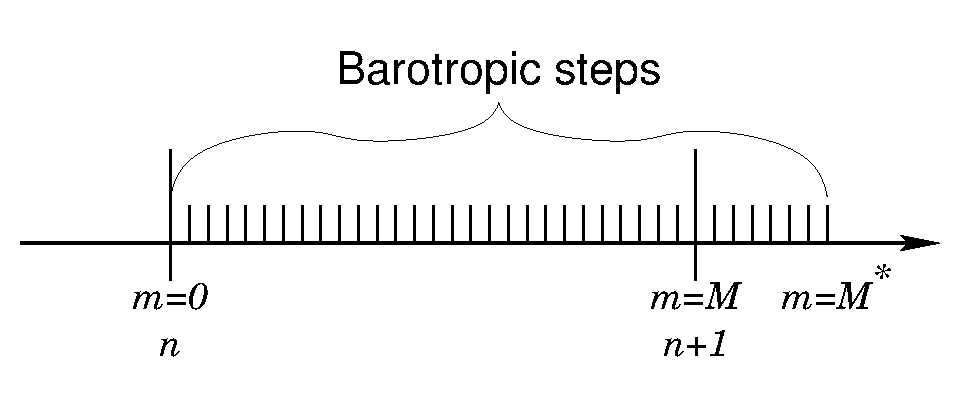
\includegraphics{pics/shortstep}%
\end{picture}%
 
 \caption{The split time stepping used in the model.}
 \label{ftspl}
\end{figure}

Some of the terms in equations (\ref{ubar1}) and (\ref{vbar1}) are
updated on the short time step while others are not.  The contributions
from the slow terms are computed once per long time step and stored.  If
we call these terms $R_{u_{\rm slow}}$ and $R_{v_{\rm slow}}$, equations
(\ref{ubar1}) and (\ref{vbar1}) become:
%{\samepage
\begin{multline}
   \frac{\partial}{\partial t} \left( \frac{D \overline{u}}{mn} \right)
   + \frac{\partial}{\partial \xi}
   \left( \frac{D \overline{u}\,\overline{u}}{n} \right)
   + \frac{\partial}{\partial \eta}
   \left( \frac{D \overline{u}\,\overline{v}}{m} \right)
   - \frac{Df\overline{v}}{mn}
\\ \vspace{1mm}
   - \left[ \overline{v}\,\overline{v}
   \frac{\partial}{\partial \xi}
   \left( \frac{1}{n} \right) - \overline{u}\,\overline{v}
   \frac{\partial}{\partial \eta} \left(
   \frac{1}{m} \right) \right] D = R_{u_{\rm slow}} -
   \frac{gD}{n} \frac{\partial \zeta}{\partial \xi}
    + \frac{D}{mn} {\cal D}_{\overline{u}}
   - \frac{1}{mn} \tau^{\xi}_b
\label{ubar2}
\end{multline}
%}  
%{\samepage
\begin{multline}
   \frac{\partial}{\partial t} \left( \frac{D \overline{v}}{mn} \right)
   + \frac{\partial}{\partial \xi}
   \left( \frac{D \overline{u}\,\overline{v}}{n} \right)
   + \frac{\partial}{\partial \eta}
   \left( \frac{D \overline{v}\,\overline{v}}{m} \right)
   + \frac{Df\overline{u}}{mn}
\\ \vspace{1mm}
   + \left[ \overline{u}\,\overline{v}
   \frac{\partial}{\partial \xi}
   \left( \frac{1}{n} \right) - \overline{u}\,\overline{u}
   \frac{\partial}{\partial \eta} \left(
   \frac{1}{m} \right) \right] D = R_{v_{\rm slow}} -
   \frac{gD}{m} \frac{\partial \zeta}{\partial \eta}
    + \frac{ D}{mn} {\cal D}_{\overline{v}}
   - \frac{1}{mn} \tau^{\eta}_b .
\label{vbar2}
\end{multline}
%}
When time stepping the model, we compute the right-hand-sides for
equations (\ref{st13}) and (\ref{st14}) as well as the
right-hand-sides for equations (\ref{ubar2}) and (\ref{vbar2}).  The
vertical integral of the 3-D right-hand-sides are obtained and then the
2-D right-hand-sides are subtracted.  The resulting fields are the slow
forcings $R_{u_{\rm slow}}$ and $R_{v_{\rm slow}}$.  This was found to
be the easiest way to retain the baroclinic contributions of the
non-linear terms such as $\overline{uu} - \overline{u}\,\overline{u}$.

The model is time stepped from time $n$ to time $n+1$ by using short
time steps on equations (\ref{ubar2}), (\ref{vbar2}) and (\ref{zeta1}).
Equation (\ref{zeta1}) is time stepped first, so that an estimate of the
new $D$ is available for the time rate of change terms
in equations (\ref{ubar2}) and (\ref{vbar2}).
A third-order predictor-corrector time stepping is used.
In practice, we actually time step all the way to time
$(n+\code{dtfast} \times M^\star)$,
while maintaining weighted averages of the values of $\overline{u}$,
$\overline{v}$ and $\zeta$.  The averages are used to replace the
values at time $n+1$ in both the baroclinic and barotropic modes,
and for recomputing the vertical grid spacing $H_z$.
Fig.~\ref{fbarostep1} shows one option for how these weights might look.

\begin{figure}[tbp]
\setlength{\unitlength}{1.in}%
\begin{picture}(6.5,6.5)(0,0)
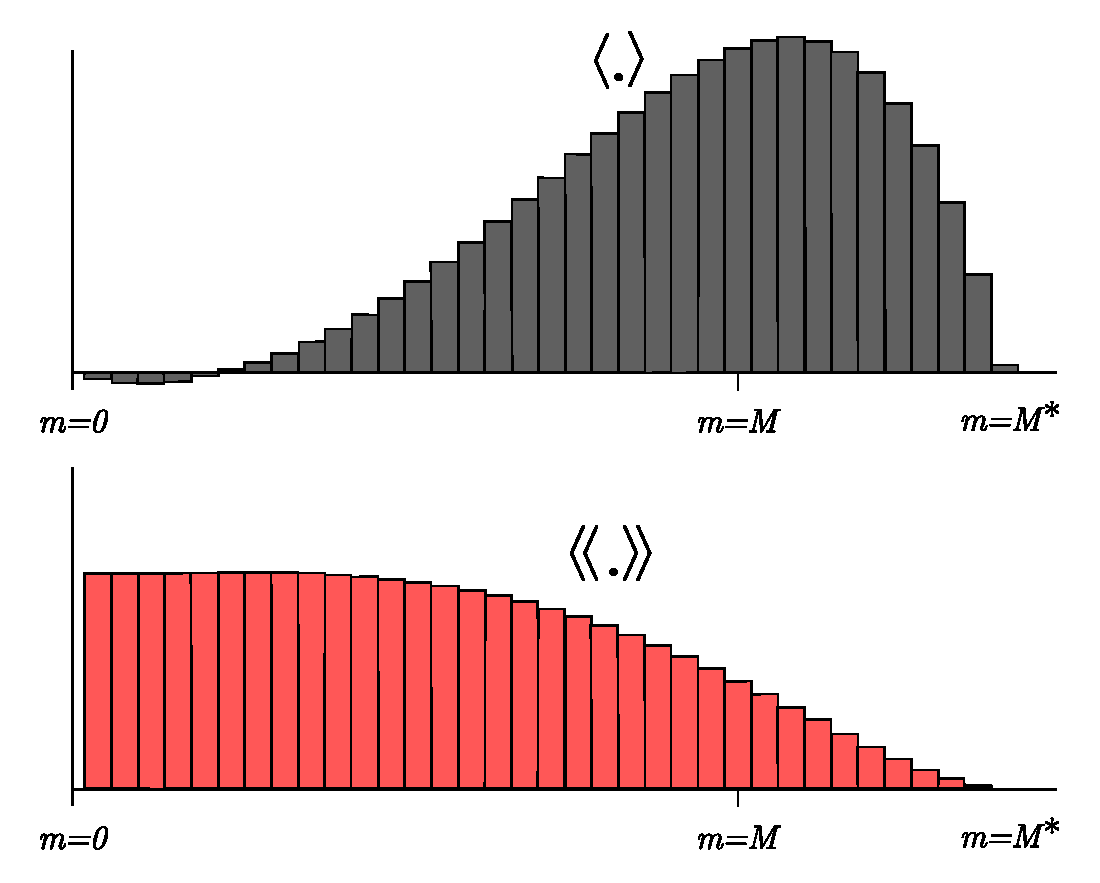
\includegraphics[width=6.5in]{pics/barostep}%
\end{picture}%
\caption{Weights for the barotropic time stepping. The upper panel
shows the primary weights, centered at time $n+1$, while the lower panel shows
the secondary weights weights, centered at time $n+\frac{1}{2}$.}
\label{fbarostep1}
\end{figure}

The primary weights, $a_m$, are used to compute $\langle \zeta
\rangle^{n+1} \equiv \sum_{m=1}^{M^\star} a_m \zeta^m$. There is a
related set of secondary weights $b_m$, used as $\langle \! \langle
\overline{u} \rangle \! \rangle^{n+\frac{1}{2}} \equiv \sum_{m=1}^{M^\star} b_m
\overline{u}^m$. In order to maintain constancy preservation, this
relation must hold:
\begin{equation}
  \langle \zeta \rangle_{i,j}^{n+1} = \langle \zeta \rangle_{i,j}^n -
  (mn)_{i,j} \Delta t \left[ \left\langle \!\! \left\langle
  \frac{D\overline u}{n} \right\rangle \!\!
  \right\rangle_{i+\frac{1}{2},j}^{n+\frac{1}{2}}
  - \left\langle \!\! \left\langle \frac{D\overline u}{n} \right\rangle
  \!\! \right\rangle_{i-\frac{1}{2},j}^{n+\frac{1}{2}} +
  \left\langle \!\! \left\langle
  \frac{D\overline v}{m} \right\rangle \!\!
  \right\rangle_{i,j+\frac{1}{2}}^{n+\frac{1}{2}}
  - \left\langle \!\! \left\langle \frac{D\overline v}{m} \right\rangle
  \!\! \right\rangle_{i,j-\frac{1}{2}}^{n+\frac{1}{2}} \right]
\label{zeta3}
\end{equation}
Shchepetkin and McWilliams (\cite{SS2005}) introduce a range of
possible weights, but the ones used here have a shape function:
\begin{equation}
   A(\tau) = A_0 \left\{ \left( \frac{\tau}{\tau_0} \right)^p \left[ 1-
   \left(\frac{\tau}{\tau_0} \right)^q \right] - r \frac{\tau}{\tau_0}
   \right\}
\label{weights}
\end{equation}
where $p, q$ are parameters and $A_0, \tau_0$, and $r$ are chosen to
satisfy normalization, consistency, and second-order accuracy
conditions,
\begin{equation}
   I_n = \int_0^{\tau^\star} \tau^n A(\tau) d \tau = 1, \quad n=0,1,2
\label{second}
\end{equation}
using Newton iterations. $\tau^\star$ is the upper limit of $\tau$
with $A(\tau) \geq 0$. In practice we initially set
$$
  A_0 = 1, r = 0 \quad \mbox{and} \quad
  \tau = \frac{(p+2)(p+q+2)}{(p+1)(p+q+1)},
$$
compute $A(\tau)$ using eq.~(\ref{weights}), normalize using:
\begin{equation}
   \sum_{m=1}^{M^\star} a_m \equiv 1, \quad
   \sum_{m=1}^{M^\star} a_m\frac{m}{M} \equiv 1,
\end{equation}
and adjust $r$ iteratively to satisfy the $n=2$ condition of
(\ref{second}). We are using values of $p=2$, $q=4$, and $r=0.284$.
This form allows some negative weights for small $m$, allowing
$M^\star$ to be less than $1.5M$.

ROMS also supports an older cosine weighting option, which isn't
recommended since it is only first-order accurate.

\subsection{Density in the mode coupling}

Equation (\ref{ubar2}) contains the term $R_{u_{\rm slow}}$,
computed as the difference between the 3-D right-hand-side and the
2-D right-hand-side. The pressure gradient therefore has the form:
\begin{equation}
   -\frac{g D}{n} \frac{\partial \zeta}{\partial \xi} +
   \left[\frac{g D}{n} \frac{\partial \zeta}{\partial \xi} + {\cal F}
   \right]
\end{equation}
where the term in square brackets is the mode coupling term and is
held fixed over all the barotropic steps and
\begin{equation}
  {\cal F} = - \frac{1}{\rho_0 n} \int_{-h}^\zeta \frac{\partial
  P}{\partial \xi} dz
\end{equation}
is the vertically integrated pressure gradient. The latter is a function
of the bathymetry, free surface gradient, and the free surface itself,
as well as the vertical distribution of density.

The disadvantage of this approach is that after the barotropic time
stepping is complete and the new free surface is substituted into
the full baroclinic pressure gradient, its vertical integral will
no longer be equal to the sum of the new surface slope term and the
original coupling term based on the old free surface. This is one
form of mode-splitting error which can lead to trouble because the
vertically integrated pressure gradient is not in balance with the
barotropic mass flux.

Instead, let us define the following:
\begin{equation}
  \overline{\rho} = \frac{1}{D} \int_{-h}^\zeta \rho dz , \quad
  \rho^\star = \frac{1}{\frac{1}{2} D^2} \int_{-h}^\zeta
  \left\{ \int_z^\zeta \rho dz^{\prime} \right\} dz
\end{equation}
Changing the vertical coordinate to $\sigma$ yields:
\begin{equation}
  \overline{\rho} =  \int_{-1}^0 \rho d\sigma , \quad
  \rho^\star = 2 \int_{-1}^0
  \left\{ \int_\sigma^0 \rho d\sigma^{\prime} \right\} d\sigma
\end{equation}
which implies that $\overline{\rho}$ and $\rho^\star$ are actually
independent of $\zeta$ as long as the density profile $\rho =
\rho(\sigma)$ does not change. The vertically integrated pressure
gradient becomes:
\begin{equation}
   -\frac{1}{\rho_0} \frac{g}{n} \left\{ \frac{\partial}{\partial \xi}
   \left( \frac{\rho^\star D^2}{2} \right) - \overline{\rho} D
   \frac{\partial h}{\partial \xi} \right\} = -\frac{1}{\rho_0}
   \frac{g}{n} D \left\{ \rho^\star \frac{\partial \zeta}{\partial \xi} +
   \frac{D}{2} \frac{\partial \rho^\star}{\partial \xi} + (\rho^\star -
   \overline{\rho}) \frac{\partial h}{\partial \xi} \right\}
\end{equation}
In the case of uniform density $\rho_0$, we obtain $\rho^\star \equiv
\overline{\rho} \equiv \rho_0$, but we otherwise have two new terms.
The accuracy of these terms depends on an accurate vertical
integration of the density, as described in Shchepetkin and
McWilliams (2005, \cite{SS2005}).

\subsection{Time stepping: internal velocity modes and tracers}
The momentum equations (\ref{st13}) and(\ref{st14}) are advanced before
the tracer equation, by computing all the terms except the vertical
viscosity and then using the implicit scheme described in \S\ref{Vfric}
to find the new values for $u$ and $v$. The depth-averaged component
is then removed and replaced by the $\langle \overline{u} \rangle$
and $\langle \overline{v} \rangle$ computed as in \S\ref{Vort}.
A third-order Adams-Bashforth (AB3) time stepping is used, requiring
multiple right-hand-side time levels (see Appendix~\ref{Frog}). These
stored up r.h.s. values can be used to extrapolate to a value at
time $n+\frac{1}{2}$ for use in the barotropic steps as shown in
Fig.~\ref{ftimestep1}.

The tracer concentration equation (\ref{tfull}) is advanced in a
predictor-corrector leapfrog-trapezoidal step, with great care taken to
optimize both the conservation and constancy-preserving properties of the
continuous equations. The corrector step can maintain both, as long as it
uses velocities and column depths which satisfy eq.~(\ref{zeta3}). This
also requires tracer values centered at time $n+\frac{1}{2}$, obtained
from the predictor step. The vertical diffusion is computed as in
\S\ref{Vfric}.

The predictor step cannot be both constancy-preserving and conservative; it
was therefore decided to make it constancy-preserving. Also, since it is
only being used to compute the advection for the corrector step, the
expensive diffusion operations are not carried out during the predictor step.

The preceeding notes on tracer advection refer to all but the MPDATA
option. The MPDATA algorithm has its own predictor-corrector with
emphasis on not allowing values to exceed their original range;
it therefore gives up the constancy-preservation. This is most
noticeable in shallow areas with large tides.

\subsection{Advection schemes}
\label{Advect}
The advection of a tracer $C$ has an equation of the form
\begin{equation}
  \frac{\partial}{\partial t} \frac{ H_z C}{mn} =
  - \frac{\partial}{\partial \xi} F^\xi
  - \frac{\partial}{\partial \eta} F^\eta
  - \frac{\partial}{\partial \sigma} F^\sigma ,
\end{equation}
where we have introduced the advective fluxes:
\begin{align}
   F^\xi &= \frac{H_z u C}{n} \\
   F^\eta &= \frac{H_z v C}{m} \\
   F^\sigma &= \frac{H_z \Omega C}{mn} .
\end{align}

\subsubsection{Second-order Centered}
The simplest form of the advective fluxes is the centered
second-order:
\begin{align}
   F^\xi &= \frac{\overline{H_z}^\xi u
               \overline{C}^\xi}{\overline{n}^\xi} \\
   F^\eta &= \frac{\overline{H_z}^\eta v
               \overline{C}^\eta}{\overline{m}^\eta} \\
   F^\sigma &= \frac{\overline{H_z}^\sigma \Omega
               \overline{C}^\sigma}{mn} .
\end{align}
This scheme is known to have some unfortunate
properties in the presence of strong gradients, such as large over- and
under-shoots of tracers, leading to the need for large amounts of
horizontal smoothing. ROMS provides alternative advection
schemes with better behavior in many situations, but retains this
one for comparison purposes.

\subsubsection{Fourth-order Centered}
The barotropic advection is centered fourth-order unless you
specifically pick centered second-order as your horizontal advection
scheme. To get fourth-order, create gradient terms:
\begin{align}
     G^{\xi} &= \overline{\left(\frac{\partial C}{\partial
            \xi}\right)}^\xi \\
     G^{\eta} &= \overline{\left(\frac{\partial C}{\partial
            \eta}\right)}^\eta \\
     G^{\sigma} &= \overline{\left(\frac{\partial C}{\partial
            \sigma}\right)}^\sigma  .
\end{align}
The fluxes now become:
\begin{align}
   F^\xi &= \frac{\overline{H_z}^\xi} {\overline{n}^\xi} u \left(
               \overline{C}^\xi -
           \frac{1}{3} \frac{\partial
               G^{\xi}}{\partial \xi} \right) \label{uflux} \\
   F^\eta &= \frac{\overline{H_z}}{\overline{m}^\eta} ^\eta v \left(
               \overline{C}^\eta-
           \frac{1}{3} \frac{\partial
               G^{\eta}}{\partial \eta} \right) \\
   F^\sigma &= \frac{\overline{H_z}^\sigma} {mn} \Omega \left(
               \overline{C}^\sigma -
           \frac{1}{3} \frac{\partial
               G^{\sigma}}{\partial \sigma} \right) \label{wflux} .
\end{align}

\subsubsection{Fourth-order Akima}
An alternate fourth-order algorithm is that by Akima:
\begin{align}
     G^{\xi} &= 2 {\frac{\partial C}{\partial \xi}_i
         \frac{\partial C}{\partial \xi}_{i+1}} \, \bigg/ \left(
         \frac{\partial C}{\partial \xi}_i +
          \frac{\partial C}{\partial \xi}_{i+1} \right) \\
     G^{\eta} &= 2 {\frac{\partial C}{\partial \eta}_j
         \frac{\partial C}{\partial \eta}_{j+1}} \, \bigg/ \left(
         \frac{\partial C}{\partial \eta}_j +
          \frac{\partial C}{\partial \eta}_{j+1} \right) \\
     G^{\sigma} &= 2 {\frac{\partial C}{\partial \sigma}_k
         \frac{\partial C}{\partial \sigma}_{k-1}} \, \bigg/ \left(
         \frac{\partial C}{\partial \sigma}_k +
          \frac{\partial C}{\partial \sigma}_{k-1} \right) \\
\end{align}
With the fluxes as in \ref{uflux}--\ref{wflux}.

\subsubsection{Third-order Upwind}
There is a class of third-order upwind advection schemes, both
one-dimensional (Leonard \cite{Leonard79}) and two-dimensional (Rasch
\cite{Rasch94} and Shchepetkin and McWilliams \cite{SS98}). This scheme
is known as UTOPIA (Uniformly Third-Order Polynomial Interpolation
Algorithm). Applying flux limiters to UTOPIA is explored in Thuburn
\cite{Thuburn96}, although it is not implemented in ROMS. The
two-dimensional formulation in Rasch contains terms of order $u^2C$
and $u^3C$, including cross terms ($uvC$). The terms which are
nonlinear in velocity have been dropped in ROMS, leaving one extra upwind
term in the computation of the advective fluxes:
\begin{align}
   F^\xi &= \frac{H_z u}{n} \left( C - \gamma \frac{\partial^2
   C}{\partial \xi^2} \right) \\
   F^\eta &= \frac{H_z v}{m} \left( C - \gamma \frac{\partial^2
   C}{\partial \eta^2} \right)
\end{align}
The second derivative terms are centered on a $\rho$ point in the grid,
but are needed at a $u$ or $v$ point in the flux. The upstream value is
used:
\begin{equation}
   F^\xi_{i,j,k} = \frac{\overline{H_z}^\xi}{\overline{n}^\xi}
   \left[ \max(0,u_{i,j,k}) C_{i-1,j,k} +
   \min(0,u_{i,j,k}) C_{i,j,k} \right] .
\label{equp}
\end{equation}
The value of $\gamma$ in the model is
$\frac{1}{8}$ while that in Rasch \cite{Rasch94} is $\frac{1}{6}$.

Because the third-order upwind scheme is designed to be
two-dimensional, it is not used in the vertical (though one might argue
that we are simply performing one-dimensional operations here).
Instead, we use a centered fourth-order scheme in the vertical when
the third-order upwind option is turned on:
\begin{equation}
   F^s = \frac{H_z w}{mn} \left[
     - \frac{1}{16} C_{i,j,k-1} + \frac{9}{16} C_{i,j,k} +
       \frac{9}{16} C_{i,j,k+1} - \frac{1}{16} C_{i,j,k+2} \right]
\end{equation}

One advantage of UTOPIA over MPDATA is that it can be used on
variables having both negative and positive values. Therefore,
it can be used on velocity as well as scalars (is there a reference for
this?). For the $u$-velocity, we have:
\begin{align}
   F^\xi &= \left(u - \gamma \frac{\partial^2 u}{\partial \xi^2} \right)
   \left[ \frac{H_z u}{n} - \gamma \frac{\partial^2}{\partial \xi^2}
   \left( \frac{H_z u}{n} \right) \right] \\
   F^\eta &= \left(u - \gamma \frac{\partial^2 u}{\partial \eta^2}
     \right)
   \left[ \frac{H_z v}{m} - \gamma \frac{\partial^2}{\partial \xi^2}
   \left( \frac{H_z v}{m} \right) \right] \\
   F^\sigma &= \frac{H_z w}{mn} \left[
     - \frac{1}{16} u_{i,j,k-1} + \frac{9}{16} u_{i,j,k} +
       \frac{9}{16} u_{i,j,k+1} - \frac{1}{16} u_{i,j,k+2} \right]
\end{align}
while for the $v$-velocity we have:
\begin{align}
   F^\xi &= \left(v - \gamma \frac{\partial^2 v}{\partial \xi^2} \right)
   \left[ \frac{H_z u}{n} - \gamma \frac{\partial^2}{\partial \eta^2}
   \left( \frac{H_z u}{n} \right) \right] \\
   F^\eta &= \left(v - \gamma \frac{\partial^2 v}{\partial \eta^2}
     \right)
   \left[ \frac{H_z v}{m} - \gamma \frac{\partial^2}{\partial \eta^2}
   \left( \frac{H_z v}{m} \right) \right] \\
   F^\sigma &= \frac{H_z w}{mn} \left[
     - \frac{1}{16} v_{i,j,k-1} + \frac{9}{16} v_{i,j,k} +
       \frac{9}{16} v_{i,j,k+1} - \frac{1}{16} v_{i,j,k+2} \right]
\end{align}
In all these terms, the second derivatives are evaluated at an upstream
location.

\subsection{Determination of the vertical velocity and density fields}
\label{EOS}
Having obtained a complete specification of the $u,v,T,$ and $S$ fields
at the next time level by the methods outlined above, the vertical
velocity and density fields can be calculated.  The vertical velocity
is obtained by combining equations (\ref{st17}) and (\ref{zeta1}) to
obtain:
\begin{equation}
   \frac{\partial}{\partial \xi} \left( \frac{H_z u}{n} \right) +
   \frac{\partial}{\partial \eta} \left( \frac{H_z v}{m} \right) +
   \frac{\partial}{\partial \sigma}\left( \frac{H_z \Omega}{mn} \right)
   - \frac{\partial}{\partial \xi} \left( \frac{D \overline{u}}{n}
   \right) -
   \frac{\partial}{\partial \eta} \left( \frac{D \overline{v}}{m}
   \right)  = 0 .
\label{zeta2}
\end{equation}
Solving for $H_z \Omega / mn$ and using the semi-discrete notation of
\S\ref{Enrg} we obtain:
\begin{equation}
   \frac{H_z \Omega}{mn} =  \int  \left[
   \delta_{\xi} \left( \frac{\overline{u} \overline{D}^{\xi}}
   {\overline{n}^{\xi}} \right) +
   \delta_{\eta} \left( \frac{\overline{v} \overline{D}^{\eta}}
   {\overline{m}^{\eta}} \right) -
   \delta_{\xi} \left( \frac{u \overline{H_z}^{\xi}}
   {\overline{n}^{\xi}} \right) - 
   \delta_{\eta} \left( \frac{v \overline{H_z}^{\eta}}
   {\overline{m}^{\eta}} \right)  \right] d\sigma .
\label{omega}
\end{equation}
The integral is actually computed as a sum from the bottom upwards and
also as a sum from the top downwards.  The value used is a linear
combination of the two, weighted so that the surface down value is used
near the surface while the other is used near the bottom.

The density is obtained from temperature and salinity via an
equation of state.  ROMS provides a choice of a nonlinear equation
of state $\rho = \rho(T,S,z)$ or a linear equation of state $\rho =
\rho(T)$.  The nonlinear equation of state has been modified and now
corresponds to the UNESCO equation of state as derived by Jackett and
McDougall \cite{Jackett}.  It computes {\sl in situ} density as a
function of potential temperature, salinity and pressure.

Warning: although we have used it quite extensively, McDougall
(personal communication) claims that the single-variable ($\rho =
\rho(T)$) equation of state is not dynamically appropriate as is.
He has worked out the extra source and sink terms required, arising
from vertical motions and the compressibility of water.  They are
quite complicated and we have not implemented them to see if they
alter the flow.

%\subsection{The pressure gradient terms}
%\label{PG}
%The pressure gradient terms in equations (\ref{st13}) and
%(\ref{st14}) are written in the form
%\begin{equation}
%  H_z \nabla \phi + \frac{g \rho H_z}{\rho_o} \nabla z
%  + g H_z \nabla \zeta
%\label{prgs}
%\end{equation}
%This is the form traditionally used in sigma-coordinate models to
%account for the horizontal differences being taken along surfaces of
%constant $\sigma$.  This form can be shown to lead to significant
%errors when $|\nabla h|$ is large (Haney \cite{Haney}; and Beckmann
%and Haidvogel \cite{BH93}). Shchepetkin....

\subsection{Horizontal mixing}
\label{Smooth}

In Chapter \ref{Phys}, the diffusive terms were written simply as
${\cal D}_u, {\cal D}_v, {\cal D}_T,$ and ${\cal D}_S$.  The vertical
component of these terms is described in \S\ref{Vfric}.  Here we
describe the ROMS options for representing the horizontal
component of these terms, first the viscosity then the diffusion.

\subsubsection{Deviatory stress tensor (viscosity)}

Note: this material was copied from the wiki, where it was
contributed by Hernan Arango. He uses ``$s$'' where we have been using
``$\sigma$'' while here $\sigma$ is the stress tensor.

The horizontal components of the divergence of the stress tensor
\citep{Wajsowicz_93} in
nondimesional, orthogonal curvilinear coordinates ($\xi$, $\eta$,
$s$) with dimensional, spatially-varying metric factors
($\frac{1}{m}$, $\frac{1}{n}$, $H_{z}$) and velocity components
($u$, $v$, $\omega H_{z}$) are given by:

\begin{align}
      F^{u} \equiv
\widehat{\xi}\cdot\left(\nabla\cdot\vec{\sigma}\right) =
          \frac{mn}{H_{z}} \Biggl[ & {\pder{}{\xi}}  \Biggl(
\frac{H_{z}{\sigma}_{\xi\xi}} {n} \Biggr) +
                                     {\pder{}{\eta}} \Biggl(
\frac{H_{z}{\sigma}_{\xi\eta}}{m} \Biggr) +
                                     {\pder{}{s}}    \Biggl(
\frac{{\sigma}_{\xi s}}{mn} \Biggr) + \\
         &H_{z}{\sigma}_{\xi\eta}  {\pder{}{\eta}} \left(
\frac{1}{m}\right) -
          H_{z}{\sigma}_{\eta\eta} {\pder{}{\xi}}  \left(
\frac{1}{n}\right) -
          \frac{1}{n} {\sigma}_{ss}{\pder{H_{z}}{\xi}} \Biggr]
\label{eqstressu}
\end{align}

\begin{align}
      F^{v} \equiv
\widehat{\eta}\cdot\left(\nabla\cdot\vec{\sigma}\right) =
          \frac{mn}{H_{z}} \Biggl[ & {\pder{}{\xi}}  \Biggl(
\frac{H_{z}{\sigma}_{\eta\xi}} {n} \Biggr) +
                                     {\pder{}{\eta}} \Biggl(
\frac{H_{z}{\sigma}_{\eta\eta}}{m} \Biggr) +
                                     {\pder{}{s}}    \Biggl(
\frac{{\sigma}_{\eta s}}{mn} \Biggr) + \\
         &H_{z}{\sigma}_{\eta\xi}  {\pder{}{\xi}}  \left(
\frac{1}{n} \right) -
          H_{z}{\sigma}_{\xi\xi}   {\pder{}{\eta}} \left(
\frac{1}{m} \right) -
          \frac{1}{m}{\sigma}_{ss} {\pder{H_{z}}{\eta}} \Biggr]
\label{eqstressv}
\end{align}

where
\begin{align}
      {\sigma}_{\xi\xi}   &= \left( A_{M} + \nu \right) e_{\xi\xi} +
\left( \nu - A_{M}\right) e_{\eta\eta}, \\
   \noalign{\smallskip}
      {\sigma}_{\eta\eta} &= \left( \nu - A_{M} \right) e_{\xi\xi} +
\left( A_{M} + \nu\right) e_{\eta\eta}, \\
   \noalign{\smallskip}
      {\sigma}_{ss} &= 2\,\nu\,e_{ss}, \\
   \noalign{\smallskip}
      {\sigma}_{\xi\eta} &= {\sigma}_{\eta\xi} =
2\,A_{M}\,e_{\xi\eta}, \\
   \noalign{\smallskip}
      {\sigma}_{\xi s}   &=  2\,K_{M}\,e_{\xi s}, \\
   \noalign{\smallskip}
      {\sigma}_{\eta s}  &=  2\,K_{M}\,e_{\eta s},
\end{align}

and the strain field is:

\begin{align}
      e_{\xi\xi}   &= m  {\pder{u}{\xi}}  + mnv {\pder{}{\eta}}
\left( \frac{1}{m} \right), \\
   \noalign{\smallskip}
      e_{\eta\eta} &= n\;{\pder{v}{\eta}} + mnu {\pder{}{\xi}}
\left( \frac{1}{n} \right), \\
   \noalign{\smallskip}
      e_{ss} &= \frac{1}{H_{z}}   {\pder{\left( \omega H_{z} \right)
}{s}} + 
                \frac{m}{H_{z}} u {\pder{H_{z}}{\xi}} +
                \frac{n}{H_{z}} v {\pder{H_{z}}{\eta}}, \\
   \noalign{\smallskip}
      2\,e_{\xi\eta} &= \frac{m}{n} {\pder{\left( nv \right) }{\xi}}
+
                        \frac{n}{m} {\pder{\left( mu \right)
}{\eta}}, \\
   \noalign{\smallskip}
      2\,e_{\xi s} &= \frac{1}{mH_{z}}  {\pder{\left( mu \right)
}{s}} +
                 m H_{z} {\pder{\omega}{\xi}}, \\
   \noalign{\smallskip}
      2\,e_{\eta s} &= \frac{1}{nH_{z}} \;
{\pder{\left(nv\right)}{s}} \;+
                 n\;H_{z} {\pder{\omega}{\eta}}.
\end{align}

Here, $A_{M}(\xi,\eta)$ and $K_{M}(\xi,\eta,s)$ are the spatially
varying horizontal and vertical viscosity coefficients,
respectively, and $\nu$ is another (very small, often neglected)
horizontal viscosity coefficient. Notice that because of the
generalized terrain-following vertical coordinates of ROMS, we need
to transform the horizontal partial derivatives from constant
''z-''surfaces to constant ''s-''surfaces.  And the vertical metric
or level thickness is the Jacobian of the transformation,
$H_{z}={\pder{z}{s}}$. Also in these models, the ''vertical''
velocity is computed as $\frac{\omega H_{z}}{mn}$ and has units of
$\hbox{m}^3/\hbox{s}$.

\subsubsection{Transverse stress tensor}

Assuming transverse isotropy, as in
\citet{Sadourny_97} and \citet{Griffies_2000},
the deviatoric stress tensor can be split into vertical and horizontal
sub-tensors.  The horizontal (or transverse) sub-tensor is symmetric, it
has a null trace, and it possesses axial symmetry in the local vertical
direction.  Then, the transverse stress tensor can be derived from eq.
(\ref{eqstressu}) and (\ref{eqstressv}), yielding

\begin{align}
      H_{z}F^{u} &= {n^2}m
{\partial\over\partial\xi}\left(\frac{H_{z}F^{u\xi}}{n}\right) +
                {m^2}n
{\partial\over\partial\eta}\left(\frac{H_{z}F^{u\eta}}{m}\right)
\label{eqtstressu} \\
   \noalign{\smallskip}
      H_{z}F^{v} &= {n^2}m
{\partial\over\partial\xi}\left(\frac{H_{z}F^{v\xi}}{n}\right) +
                {m^2}n
{\partial\over\partial\eta}\left(\frac{H_{z}F^{v\eta}}{m}\right)
\label{eqtstressv} 
\end{align}

where

\begin{align}
         F^{u\xi} &= \frac{1}{n} \;A_{M}\left[
               \frac{m}{n} {\pder{\left( nu \right) }{\xi}} \;-
               \frac{n}{m} {\pder{\left( mv \right) }{\eta}}
\right], \\
      \noalign{\smallskip}
         F^{u\eta} &= \frac{1}{m} A_{M}\left[
               \frac{n}{m} {\pder{\left( mu \right) }{\eta}} +
               \frac{m}{n} {\pder{\left( nv \right) }{\xi}}
\;\right], \\
      \noalign{\medskip}
         F^{v\xi} &= \frac{1}{n} \;A_{M}\left[
               \frac{m}{n} {\pder{\left( nv \right) }{\xi}} \;+
               \frac{n}{m} {\pder{\left( mu \right) }{\eta}}
\right], \\
      \noalign{\smallskip}
         F^{v\eta} &= \frac{1}{m} A_{M}\left[
               \frac{n}{m} {\pder{\left( mv \right) }{\eta}} -
               \frac{m}{n} {\pder{\left( nu \right) }{\xi}}
\;\right].
\end{align}

Notice the flux form of eq. (\ref{eqtstressu}) and (\ref{eqtstressv})
and the symmetry between the $F^{u\xi}$ and $F^{v\eta}$ terms which are
defined at density points on a C-grid. Similarly, the $F^{u\eta}$ and
$F^{v\xi}$ terms are symmetric and defined at vorticity points.  These
staggering positions are optimal for the discretization of the tensor;
it has no computational modes and satisfies first-moment conservation.

The biharmonic friction operator can be computed by applying the tensor
operator eq. (\ref{eqtstressu}) and (\ref{eqtstressv}) twice, but with
the squared root of the biharmonic viscosity coefficient
\citep{Griffies_2000}.  For simplicity and momentum
balance, the thickness $H_{z}$ appears only when computing the second
harmonic operator as in \citet{Griffies_2000}.

\subsubsection{Rotated Transverse Stress Tensor}

In some applications with tall and steep topography, it
will be advantageous to substantially reduce the contribution of the
stress tensor eq. (\ref{eqtstressu}) and (\ref{eqtstressv}) to
the vertical mixing when operating along constant $s$-surfaces.
The transverse stress tensor rotated along geopotentials (constant depth)
is then given by

\begin{align}
      H_{z}R^{u} &= {n^2}m {\pder{}{\xi}}  \Biggl(
\frac{H_{z}R^{u\xi}} {n} \Biggr) +
                    {m^2}n {\pder{}{\eta}} \Biggl(
\frac{H_{z}R^{u\eta}}{m} \Biggr) +
                           {\pder{}{s}}    \Biggl( R^{us} \Biggr)
\label{eqrstressu}
\\
   \noalign{\smallskip}
      H_{z}R^{v} &= {n^2}m {\pder{}{\xi}}  \Biggl(
\frac{H_{z}R^{v\xi}} {n} \Biggr) +
                    {m^2}n {\pder{}{\eta}} \Biggl(
\frac{H_{z}R^{v\eta}}{m} \Biggr) +
                           {\pder{}{s}}    \Biggl( R^{vs} \Biggr)
\label{eqrstressv}
\end{align}

where

\begin{align}
         R^{u\xi} = &\frac{1}{n}\; A_{M} \left[
                 \frac{1}{n}\;\left( m {\pder{\left(nu\right)}{\xi}} -
                                     m {\pder{z}{\xi}} \frac{1}{H_{z}}
                         {\pder{\left( nu \right) }{s}} \right) -
                 \frac{1}{m}  \left( n {\pder{\left( mv \right) }{\eta}} -
                                     n {\pder{z}{\eta}} \frac{1}{H_{z}}
                                       {\pder{\left( mv \right) }{s}}\right)
                              \right], \\
      \noalign{\medskip}
         R^{u\eta} = &\frac{1}{m} A_{M} \left[
                 \frac{1}{m}  \left( n {\pder{\left( mu \right) }{\eta}} -
                                     n {\pder{z}{\eta}} \frac{1}{H_{z}}
                         {\pder{\left( mu \right) }{s}} \right) +
                 \frac{1}{n}\;\left( m {\pder{\left( nv \right) }{\xi}} -
                                     m {\pder{z}{\xi}} \frac{1}{H_{z}}
                                      {\pder{\left( nv \right) }{s}} \right)
                              \right], \\
      \noalign{\medskip}
         R^{us} = &m {\pder{z}{\xi}} A_{M} \left[
                 \frac{1}{n}\;\left( m {\pder{z}{\xi}} \frac{1}{H_{z}}
                                       {\pder{\left( nu \right) }{s}} -
                 m {\pder{\left( nu \right) }{\xi}} \right) -
                 \frac{1}{m}  \left( n {\pder{z}{\eta}} \frac{1}{H_{z}}
                                       {\pder{\left( mv \right) }{s}} -
                           n {\pder{\left( mv \right) }{\eta}} \right)
                              \right] +\\
                &n\; {\pder{z}{\eta}} A_{M} \left[
                 \frac{1}{m}  \left( n {\pder{z}{\eta}} \frac{1}{H_{z}}
                                       {\pder{\left( mu \right) }{s}} -
                             n {\pder{\left( mu \right) }{\eta}} \right) +
                 \frac{1}{n}\;\left( m {\pder{z}{\xi}} \frac{1}{H_{z}}
                                       {\pder{\left( nv \right) }{s}} -
                             m {\pder{\left( nv \right) }{\xi}} \right)
                              \right], \\
      \noalign{\bigskip}
         R^{v\xi} = &\frac{1}{n}\;A_{M} \left[
                 \frac{1}{n}\;\left( m {\pder{\left( nv \right) }{\xi}} -
                                     m {\pder{z}{\xi}} \frac{1}{H_{z}}
                            {\pder{\left( nv \right) }{s}} \right) +
                 \frac{1}{m}  \left( n {\pder{\left( mu \right) }{\eta}}-
                                     n {\pder{z}{\eta}} \frac{1}{H_{z}}
                                      {\pder{\left( mu \right) }{s}} \right)
                              \right], \\
      \noalign{\medskip}
         R^{v\eta} = &\frac{1}{m}A_{M} \left[
                 \frac{1}{m}  \left( n {\pder{\left( mv \right) }{\eta}} -
                                     n {\pder{z}{\eta}} \frac{1}{H_{z}}
                              {\pder{\left( mv \right) }{s}} \right) -
                 \frac{1}{n}\;\left( m {\pder{\left( nu \right) }{\xi}} -
                                     m {\pder{z}{\xi}} \frac{1}{H_{z}}
                                       {\pder{\left( nu \right)}{s}} \right)
                              \right], \\
      \noalign{\medskip}
         R^{vs} = &m {\pder{z}{\xi}} A_{M} \left[
                 \frac{1}{n}\;\left( m {\pder{z}{\xi}} \frac{1}{H_{z}}
                                       {\pder{\left( nv \right) }{s}} -
                        m {\pder{\left( nv \right) }{\xi}} \right) +
                 \frac{1}{m}  \left( n {\pder{z}{\eta}} \frac{1}{H_{z}}
                                       {\pder{\left( mu \right) }{s}} -
                            n {\pder{\left( mu \right) }{\eta}} \right)
                              \right] +\\
                &n\; {\pder{z}{\eta}} A_{M} \left[
                 \frac{1}{m}  \left( n {\pder{z}{\eta}} \frac{1}{H_{z}}
                                       {\pder{\left( mv \right) }{s}} -
                              n {\pder{\left( mv \right) }{\eta}} \right) -
                 \frac{1}{n}\;\left( m {\pder{z}{\xi}} \frac{1}{H_{z}}
                                       {\pder{\left( nu \right) }{s}} -
                            m {\pder{\left( nu \right) }{\xi}} \right)
                              \right].
\end{align}

Notice that the transverse stress tensor remains invariant under
coordinate transformation.  The rotated tensor (\ref{eqrstressu})
and (\ref{eqrstressv}) retains the
same properties as the unrotated tensor (\ref{eqtstressu}) and
(\ref{eqtstressv}).  The additional terms
that arise from the slopes of $s$-surfaces along
geopotentials are discretized using a modified version of the triad
approach of \citet{Griffies_98}.

\subsubsection{Horizontal diffusion}
\label{Smooth_diff}

In Chapter \ref{Phys}, the diffusive terms were written simply as
${\cal D}_T$ and ${\cal D}_S$. The vertical component of these terms
is described in \S\ref{Vfric}. Here we describe the various options
for representing the horizontal component of these terms.

\subsubsection{Laplacian}
The Laplacian of a scalar $C$ in curvilinear coordinates is (see
Appendix \ref{Curve}):
\begin{equation}
   \nabla^2 C = \nabla \cdot \nabla C = mn \left[ 
   {\partial \over \partial \xi} \!\! \left( {m \over n} 
   {\partial C \over \partial \xi} \right) +
   {\partial \over \partial \eta} \!\! \left( {n \over m} 
   {\partial C \over \partial \eta} \right) \right]
\end{equation}
In ROMS, this term is multiplied by ${\nu_2 H_z \over mn}$ and becomes
\begin{equation}
   \left[ 
   {\partial \over \partial \xi} \!\! \left( {\nu_2 H_zm \over n} 
   {\partial C \over \partial \xi} \right) +
   {\partial \over \partial \eta} \!\! \left( {\nu_2 H_zn \over m} 
   {\partial C \over \partial \eta} \right) \right]
\end{equation}
where $C$ is any tracer. This form guarantees
that the term does not contribute to the volume-integrated equations.

\subsubsection{Biharmonic}
The biharmonic operator is $\nabla^4 = \nabla^2 \nabla^2$; the
corresponding term is computed using a temporary variable $Y$:
\begin{equation}
   Y =
   {mn \over H_z} \left[ 
   {\partial \over \partial \xi} \!\! \left( {\nu_4 H_zm \over n} 
   {\partial C \over \partial \xi} \right) +
   {\partial \over \partial \eta} \!\! \left( {\nu_4 H_zn \over m} 
   {\partial C \over \partial \eta} \right) \right]
\end{equation}
and is
\begin{equation}
   - \left[ 
   {\partial \over \partial \xi} \!\! \left( {\nu_4 H_zm \over n} 
   {\partial Y \over \partial \xi} \right) +
   {\partial \over \partial \eta} \!\! \left( {\nu_4 H_zn \over m} 
   {\partial Y \over \partial \eta} \right) \right]
\end{equation}
where $C$ is once again any tracer and $\nu_4$ is the square root of
the input value so that it can be applied twice.

\subsubsection{Rotated mixing tensors}
Both the Laplacian and biharmonic terms above operate on surfaces of
constant $s$ and can contribute substantially to the vertical mixing.
However, the oceans are thought to mix along constant density surfaces so
this is not entirely satisfactory. Therefore, the option of using rotated
mixing tensors for the Laplacian and biharmonic operators has been added.
Options exist to diffuse on constant $z$ surfaces (\code{MIX\_GEO\_TS})
and constant potential density surfaces (\code{MIX\_ISO\_TS}).

The horizontal Laplacian diffusion operator is computed by finding the
three components of the flux of the quantity $C$.  The $\xi$ and
$\eta$ components are locally horizontal, rather than along the
$s$ surface. The diffusive fluxes are:
\begin{align}
   F^\xi & = \nu_2 \left[ m
   {\partial C \over \partial \xi} -
   \underbrace{ \left( m {\partial z \over \partial \xi}
   \underbrace{+ S_x }_{\mbox{\tt MIX\_ISO}} \right)
   {\partial C \over \partial z} }_{\mbox{\tt MIX\_GEO}} \right]
\label{fluxx}
\\
   F^\eta & = \nu_2 \left[ n
   {\partial C \over \partial \eta} -
   \underbrace{ \left[ n {\partial z \over \partial \eta}
   \underbrace{+ S_y }_{\mbox{\tt MIX\_ISO}} \right)
   {\partial C \over \partial z} }_{\mbox{\tt MIX\_GEO}} \right]
\label{fluxy}
\\
   F^s & =
   - \underbrace{ {1 \over H_z} \left( m
   {\partial z \over \partial \xi}
   \underbrace{+ S_x }_{\mbox{\tt MIX\_ISO}} \right)
   F^\xi }_{\mbox{\tt MIX\_GEO}}
   - \underbrace{ {1 \over H_z} \left( n
   {\partial z \over \partial \eta}
   \underbrace{+ S_y }_{\mbox{\tt MIX\_ISO}} \right)
   F^\eta }_{\mbox{\tt MIX\_GEO}}
\label{fluxs}
\end{align}
where
\begin{align*}
  S_x & = { { \partial \rho \over \partial x} \over
    { \partial \rho \over \partial z} } =
    { \left[ m {\partial \rho \over \partial \xi} -
    {m \over H_z} {\partial z \over \partial \xi}
    { \partial \rho \over \partial s} \right] \over
    {1 \over H_z} {\partial \rho \over \partial s} }
\\
  S_y & = { { \partial \rho \over \partial y} \over
    { \partial \rho \over \partial z} } =
    { \left[ n {\partial \rho \over \partial \eta} -
    {n \over H_z} {\partial z \over \partial \eta}
    { \partial \rho \over \partial s} \right] \over
    {1 \over H_z} {\partial \rho \over \partial s} }
\end{align*}
and there is some trickery whereby the computational details depend on the sign
of $\partial z \over \partial \xi$ and of $\partial z \over \partial
\eta$.  No flux boundary conditions are easily imposed by setting
\begin{eqnarray*}
  F^\xi = 0    && \mbox{ at $\xi$ walls} \\
  F^\eta = 0   && \mbox{ at $\eta$ walls} \\
  F^s = 0 && \mbox{ at $s = -1,0$}
\end{eqnarray*}

Finally, the flux divergence is calculated and is added to the
right-hand-side term for the field being computed:
\begin{equation}
  {\partial \over \partial \xi} \left( { H_z F^\xi \over n} \right) +
  {\partial \over \partial \eta} \left( { H_z F^\eta \over m} \right) +
  {\partial \over \partial s}
  \left( { H_z F^s \over mn} \right)
\label{rot1}
\end{equation}

The biharmonic rotated mixing tensors are computed much as the
non-rotated biharmonic mixing.  We define a temporary variable $Y$
based on equation (\ref{rot1}):
\begin{equation}
  Y = {mn \over H_z} \left[
  {\partial \over \partial \xi} \left( {\nu_4 H_z F^\xi \over n} \right) +
  {\partial \over \partial \eta} \left( {\nu_4 H_z F^\eta \over m} \right) +
  {\partial \over \partial s}
  \left( {\nu_4 H_z F^s \over mn} \right)
  \right] .
\end{equation}
We then build up fluxes of $Y$ as in equations
(\ref{fluxx})--(\ref{fluxs}).  We then apply equation (\ref{rot1})
to these $Y$ fluxes to obtain the biharmonic mixing tensors. Again, the
value of $\nu_4$ is the square root of that read in so that it can be
applied twice.

\subsection{Vertical mixing schemes}
\label{Vmix}
ROMS contains a variety of methods for setting the vertical viscous and
diffusive coefficients. The choices range from simply choosing fixed
values to the K-profile Parameterization (KPP) of \citet{Large94},
generic lengthscale (GLS) and Mellor-Yamada turbulence
closure schemes.  See \citet{Large98} for a review of surface ocean
mixing schemes.  Many schemes have a background molecular value which
is used when the turbulent processes are assumed to be small (such as
in the interior). All assume that there is some $K_m(\zeta,\eta,s)$
such that the vertical turbulent mixing can be applied as:
\begin{equation}
    \overline{u' w'} = -K_m {\partial u \over \partial z}
    \mbox{\quad and \quad}
    \overline{v' w'} = -K_m {\partial v \over \partial z}
\end{equation}
with a similar $K_s$ for temperature, salinity and other tracers. The
primed quantities represent perturbations of smaller scale than those
resolved by the model while the unprimed $u$ and $v$ are those in
the model.

\subsubsection{The Large, McWilliams and Doney parameterization}
\label{sec:origLMD}

The vertical mixing parameterization introduced by
\citet{Large94} is a versatile first order scheme which has
been shown to perform well in open ocean settings.  Its design
facilitates experimentation with additional or modified representations
of specific turbulent processes.

\paragraph{Surface boundary layer}
The Large, McWilliams and Doney scheme (LMD, also known as KPP)
matches separate parameterizations for vertical mixing
of the surface boundary layer and the ocean interior.  A formulation
based on boundary layer similarity theory is applied in the water
column above a calculated boundary layer depth $h_{sbl}$.  This
parameterization is then matched at the interior with schemes to
account for local shear, internal wave and double diffusive mixing
effects.  

Viscosity and diffusivities at model levels above a calculated
surface boundary layer depth ($h_{sbl}$ ) are expressed as the product
of the length scale $h_{sbl}$, a turbulent velocity scale $w_x$ and a
non-dimensional shape function.
\begin{equation}
\nu_x = h_{sbl} w_x(\sigma)G_x(\sigma)
\end{equation}
where $\sigma$ is a non-dimensional coordinate ranging from 0 to 1
indicating depth within the surface boundary layer. The $x$ subscript
stands for one of momentum, temperature and salinity.

\subparagraph{Surface Boundary layer depth}
The boundary layer depth $h_{sbl}$ is calculated as the minimum of the
Ekman depth, estimated as,
\begin{equation}
h_e=0.7u_*/f
\end{equation}
(where $u_*$ is the friction velocity $u_*=\sqrt{\tau_x^2+\tau_y^2}/\rho$ ),
 the Monin-Obukhov depth:
\begin{equation}
L=u_*^3/(\kappa B_f)
\end{equation}
(where $\kappa = 0.4$ is von Karman's contant and $B_f$ is the surface
buoyancy flux), and the shallowest depth at which a critical bulk
Richardson number is reached. The critical bulk Richardson number
($Ri_c$) is typically in the range 0.25--0.5. The bulk Richardson
number ($Ri_b$) is calculated as:
\begin{equation}
Ri_b(z)=\frac{(B_r-B(d))d}{|\vec{V}_r-\vec{V}(d)|^2+{V_t}^2(d)}
\end{equation}
where $d$ is distance down from the surface, $B$ is the buoyancy,
$B_r$ is the buoyancy at a near surface reference depth, $\vec{V}$ is
the mean horizontal velocity, $\vec{V}_r$ the velocity at the near
surface reference depth and $V_t$ is an estimate of the turbulent
velocity contribution to velocity shear.

The turbulent velocity shear term in this equation is given by LMD as,
\begin{equation}
  V_{t}^{2}(d)=\frac{C_v(-\beta_T)^{1/2}}{Ri_c
  \kappa}(c_s\epsilon)^{-1/2}dNw_s
  \label{eqtvs}
\end{equation}
where $C_v$ is the ratio of interior $N$ to $N$ at the entrainment
depth, $\beta_T$ is ratio of entrainment flux to surface buoyancy flux,
$c_s$ and $\epsilon$ are constants, and $w_s$ is the turbulent velocity
scale for scalars.
LMD derive (\ref{eqtvs}) based on the expected behavior in the pure
convective limit.  The empirical rule of convection states that the
ratio of the surface buoyancy flux to that at the entrainment depth be 
a constant.  Thus the entrainment flux at the
bottom of the boundary layer under such conditions should be
independent of the stratification at that depth.  Without a turbulent
shear term in the denominator of the bulk Richardson number
calculation, the estimated boundary layer depth is too shallow and the
diffusivity at the entrainment depth is too low to obtain the
necessary entrainment flux.  Thus by adding a turbulent shear term
proportional to the stratification in the denominator, the calculated
boundary layer depth will be deeper and will lead to a high enough
diffusivity to satisfy the empirical rule of convection.
  
\subparagraph{Turbulent velocity scale}
To estimate $w_x$ (where $x$ is $m$ - momentum {\em or} $s$
- any scalar) throughout the boundary layer, surface layer similarity
theory is utilized.  Following an argument by
\citet{TM86}, \citet{Large94} estimate the velocity scale as
\begin{equation}
w_x=\frac{\kappa u_*}{\phi_x(\zeta)}
\end{equation}
where $\zeta$ is the surface layer stability parameter defined as
$z/L$.  $\phi_x$ is a non-dimensional flux profile which varies based
on the stability of the boundary layer forcing.  The stability
parameter used in this equation is assumed to vary over the entire
depth of the boundary layer in stable and neutral conditions.  In
unstable conditions it is assumed only to vary through the surface
layer which is defined as $ \epsilon h_{sbl} $ (where $\epsilon$ is
set at 0.10) .  Beyond this depth $\zeta$
is set equal to its value at $ \epsilon h_{sbl} $.

The flux profiles are expressed as analytical fits to atmospheric
surface boundary layer data.  In stable conditions they vary linearly
with the stability parameter $\zeta$  as
\begin{equation}
\phi_x=1+5\zeta
\end{equation}
In near-neutral unstable conditions common Businger-Dyer forms are
used which match with the formulation for stable conditions at
$\zeta=0$.  Near neutral conditions are defined as 
\begin{equation}
-0.2 \leq \zeta < 0
\end{equation}
for momentum and,
\begin{equation}
-1.0 \leq \zeta < 0
\end{equation}
for scalars.  The non dimensional flux profiles in this regime are,
\begin{align}
\phi_m & =(1-16\zeta)^{1/4}
\\ \vspace{1mm}
\phi_s & =(1-16\zeta)^{1/2}
\end{align}
In more unstable conditions $\phi_x$ is chosen to match the
Businger-Dyer forms and with the free convective limit.  Here the flux 
profiles are 
\begin{align}
\phi_m & =(1.26-8.38\zeta)^{1/3}
\\ \vspace{1mm}
\phi_s & =(-28.86-98.96\zeta)^{1/3}
\end{align}

\subparagraph{The shape function}
The non-dimensional shape function $G(\sigma)$ is a third order
polynomial with coefficients chosen to match the interior viscosity at
the bottom of the boundary layer and Monin-Obukhov
similarity theory approaching the surface.  This function is defined
as a 3rd order polynomial.
\begin{equation}
G(\sigma)=a_o+a_1\sigma+a_2\sigma^2+a_3\sigma^3
\end{equation}
with the coefficients specified to match surface boundary conditions
and to smoothly blend with the interior,
\begin{align}
  a_o & =0
\\ \vspace{1mm}
  a_1 & =1
\\ \vspace{1mm}
  a_2 & =-2+3\frac{\nu_{x}(h_{sbl})}{hw_x(1)}+\frac{\partial_x
  \nu_{x}(h)}{w_{x}(1)}+\frac{\nu_{x}(h)
  \partial_{\sigma}w_x(1)}{hw_{x}^{2}(1)}
\\ \vspace{1mm}
  a_3 & =1-2\frac{\nu_{x}(h_{sbl})}{hw_x(1)}-\frac{\partial_x
  \nu_{x}(h)}{w_{x}(1)}-\frac{\nu_{x}(h)
  \partial_{\sigma}w_x(1)}{hw_{x}^{2}(1)}
\end{align}
where $\nu_{x}(h)$ is the viscosity calculated by the interior
parameterization at the boundary layer depth.

\paragraph{Countergradient flux term}
The second term of the LMD scheme's surface boundary layer
formulation is the non-local transport term $\gamma$ which can play a
significant role in mixing during surface cooling events.  This is a
redistribution term included in the tracer equation separate from the
diffusion term and is written as 
\begin{equation}
-\frac{\partial}{\partial z}K\gamma.
\end{equation}

LMD base their formulation for non-local scalar transport on a
parameterization for pure free convection from
\citet{Mailhot82}. They extend this parameterization to cover any
unstable surface forcing conditions to give
\begin{equation}
  \gamma_{T}=C_s\frac{\overline{wT_0}+
  \overline{wT_R}}{w_T(\sigma)h}
\end{equation}
for temperature and 
\begin{equation}
\gamma_S=C_s \frac{\overline{wS_0}}{w_S(\sigma)h}
\end{equation}
for salinity (other scalar quantities with surface fluxes can be
treated similarly). LMD argue that although there is evidence of
non-local transport of momentum as well, the form the term would take
is unclear so they simply specify $\gamma_m=0$.

\paragraph{The interior scheme}
The interior scheme of Large, McWilliams and Doney estimates the
viscosity coefficient by adding the effects of several generating
mechanisms:  shear mixing, double-diffusive mixing and internal wave
generated mixing.
\begin{equation}
\nu_{x}(d)=\nu_{x}^s+\nu_{x}^d+\nu_{x}^w
\end{equation}

\subparagraph{Shear generated mixing}
The shear mixing term is calculated using a
gradient Richardson number formulation,
with viscosity estimated as: 
\begin{equation}
\nu^s_x=\begin{cases}
\nu_0&   \text{$ Ri_g<0$}, \\
\nu_0[1-(Ri_g/Ri_0)^2]^3&  \text{$0< Ri_g<Ri_0$},  \\
0&   \text{$Ri_g>Ri_0$}.  
\end{cases}
\end{equation}
where $\nu_0$ is $5.0 \times 10^{-3} m^2/s$, $Ri_0 = 0.7$.  

\subparagraph{Double diffusive processes}
The second component of the interior mixing parameterization represents
double diffusive mixing.  From limited sources of laboratory and field
data LMD parameterize the salt fingering case ($R_{\rho}>1.0$)
\begin{align}
\nu_{s}^{d}(R_{\rho}) & =
	\begin{cases}
      1\times10^{-4}[1-(\frac{(R_{\rho}-1}{R_{\rho}^0-1})^2)^{3}&
      \text{for $1.0<R_{\rho}<R_{\rho}^0=1.9$},\\
           0& \text{otherwise}.
        \end{cases}
\\ \vspace{1mm}
\nu_{\theta}^{d}(R_{\rho}) & =0.7\nu_{s}^{d}
\end{align}

For diffusive convection ($0<R_{\rho}<1.0$) LMD suggest several
formulations from the literature and choose the one with the most
significant impact on mixing \citep{Fedorov88}.
\begin{equation}
\nu_{\theta}^{d}=(1.5 \time 10^{-6})(0.909 \exp(4.6 \exp[-0.54(R_{\rho}^{-1}-1)])
\end{equation}
for temperature.  For other scalars,
\begin{equation}
   \nu_{s}^{d}=
	\begin{cases}
	     \nu_{\theta}^{d}(1.85-0.85R_{\rho}^{-1})R_{\rho}& \text{for $0.5<=R_{\rho}<1.0$},\\ 
             \nu_{\theta}^{d}0.15R_{\rho}&  \text{otherwise}. \\
        \end{cases}
\end{equation}

\subparagraph{Internal wave generated mixing}
Internal wave generated mixing serves as the background mixing in the
LMD scheme.  It is specified as a constant for both scalars and
momentum.  Eddy diffusivity is estimated based on the data of
\citet{LWL93}.  While \citet{Peters88} suggest
eddy viscosity should be 7 to 10 times larger than diffusivity for
gradient Richardson numbers below approximately 0.7.  Therefore LMD use
\begin{align}
\nu_{m}^w & =1.0 \times 10^{-4} m^2 s^{-1}
\\ \vspace{1mm}
\nu_{s}^w & =1.0 \times 10^{-5} m^2 s^{-1}
\end{align}

\subsubsection{Mellor-Yamada}
\label{sec:MY25}
One of the more popular closure schemes is that of
\citet{Mellor74, Mellor82}. They actually present a hierarchy of
closures of increasing complexity. ROMS provides only the
``Level 2.5'' closure with the \citet{Galperin88}
modifications as described in \citet{Allen95}.
This closure scheme adds two prognostic equations, one
for the turbulent kinetic energy (${1 \over 2} q^2$) and one for the
turbulent kinetic energy times a length scale ($q^2l$).

The turbulent kinetic energy equation is:
\begin{equation}
  {D \over Dt} \left( {q^2 \over 2} \right) -
  {\partial \over \partial z} \left[ K_q {\partial \over \partial z} 
  \left( {q^2 \over 2} \right) \right] = P_s + P_b - \xi_d
  \label{eq:tke1}
\end{equation}
where $P_s$ is the shear production, $P_b$ is the buoyant production
and $\xi_d$ is the dissipation of turbulent kinetic energy. 
These terms are given by
\begin{align}
   P_s &= K_m \left[ \left( {\partial u \over \partial z }\right)^2 +
   \left( {\partial v \over \partial z} \right)^2 \right],  \\
   P_b &= -K_s N^2, \\
   \xi_d &= {q^3 \over B_1 l}
\end{align}
where $B_1$ is a constant.
One can also add a traditional horizontal Laplacian or biharmonic
diffusion (${\cal D}_q$) to the turbulent kinetic energy equation.
The form of this equation in the model coordinates becomes
%{\samepage
\begin{multline}
  {\partial \over \partial t} \left( {H_z q^2 \over mn} \right) +
  {\partial \over \partial \xi} \left( {H_z u q^2 \over n} \right) +
  {\partial \over \partial \eta} \left( {H_z v q^2 \over m} \right) +
  {\partial \over \partial s} \left( {H_z \Omega q^2 \over mn} \right) -
  {\partial \over \partial s} \left( {K_q \over mnH_z}
  {\partial q^2 \over \partial s} \right) =
\\ \vspace{1mm}
  {2H_z K_m \over mn} \left[ \left({\partial u \over \partial z}
  \right)^2 + \left( {\partial v \over \partial z} \right)^2 \right] +
  {2H_z K_s \over mn} N^2 - {2H_z q^3 \over mnB_1 l} +
  {H_z \over mn} {\cal D}_q .
  \label{eq:tke2}
\end{multline}
%}
The vertical boundary conditions are:
\[
\begin{array}{rl}
  \mbox{top ($z = \zeta(x,y,t))$} \hspace{1cm}
  & {H_z \Omega \over mn} = 0 \\ [1.5mm]
  & {K_q \over mn H_z} \, \frac{\partial q^2}{\partial s}
    = {B_1^{2/3} \over \rho_o} \left[ \left( \tau_s^\xi \right)^2
    + \left( \tau_s^\eta \right)^2  \right] \\ [1.5mm]
  & H_z K_m \left( {\partial u \over \partial z},
    {\partial v \over \partial z} \right) = {1 \over \rho_o}
    \left( \tau_s^\xi, \tau_s^\eta \right) \\ [1.5mm]
  & H_z K_s N^2 = {Q \over \rho_o c_P} \\[2mm]
  \mbox{and bottom ($z = -h(x,y)$)} \hspace{1cm} &
    {H_z \Omega \over mn} = 0 \\[1.5mm]
  & {K_q \over mnH_z} {\partial q^2 \over \partial s}
    = {B_1^{2/3} \over \rho_o} \left[ \left( \tau_b^\xi \right)^2
    + \left( \tau_b^\eta \right)^2  \right] \\ [1.5mm]
  & H_z K_m \left( {\partial u \over \partial z},
    {\partial v \over \partial z} \right) = {1 \over \rho_o}
    \left( \tau_b^\xi, \tau_b^\eta \right) \\ [1.5mm]
  & H_z K_s N^2 = 0
\end{array}
\]

There is also an equation for the turbulent length scale $l$:
\begin{equation}
  {D \over Dt} \left( {lq^2} \right) -
  {\partial \over \partial z} \left[ K_l
  {\partial lq^2 \over \partial z} 
  \right] = lE_1 ( P_s + P_b ) - {q^3 \over B_1} \tilde{W}
\end{equation}
where $\tilde{W}$ is the wall proximity function:
\begin{align}
  \tilde{W} &= 1 + E_2 \left( {l \over kL} \right) ^2 \\
  L^{-1} &= {1 \over \zeta -z} + {1 \over H+z}
\end{align}
The form of this equation in the model coordinates becomes
%{\samepage
\begin{multline}
  {\partial \over \partial t} \left( {H_z q^2l \over mn} \right) +
  {\partial \over \partial \xi} \left( {H_z u q^2l \over n} \right) +
  {\partial \over \partial \eta} \left( {H_z v q^2l \over m} \right) +
  {\partial \over \partial s} \left( {H_z \Omega q^2l \over mn} \right) -
  {\partial \over \partial s} \left( {K_q \over mnH_z}
  {\partial q^2l \over \partial s} \right) =
\\ \vspace{1mm}
  {H_z \over mn} lE_1 ( P_s + P_b) - 
  {H_z q^3 \over mnB_1 } \tilde{W} +
  {H_z \over mn} {\cal D}_{ql} .
  \label{eq:kkl}
\end{multline}
%}
where ${\cal D}_{ql}$ is the horizontal diffusion of the quantity
$q^2l$. Both equations (\ref{eq:tke2}) and (\ref{eq:kkl}) are timestepped
much like the model tracer equations, including an implicit solve for
the vertical operations and options for centered second and fourth-order
advection. They are timestepped with a predictor-corrector scheme in
which the predictor step is only computing the advection.

Given these solutions for $q$ and $l$, the vertical viscosity and
diffusivity coefficients are:
\begin{align}
  K_m &= qlS_m + K_{m_{\rm background}} \\
  K_s &= qlS_h + K_{s_{\rm background}} \\
  K_q &= qlS_q + K_{q_{\rm background}}
\end{align}
and the stability coefficients $S_m$, $S_h$ and $S_q$ are found by
solving
\begin{gather}
  S_s \left[ 1 - (3A_2 B_2 + 18 A_1 A_2) G_h \right] =
  A_2 \left[ 1 - 6A_1 B_1^{-1} \right]
\\ \vspace{1mm}
  S_m \left[ 1 - 9A_1 A_2 G_h \right] - S_s \left[ G_h ( 18 A_1^2 +
  9A_1 A_2 ) G_h \right] =
  A_1 \left[ 1 - 3C_1 - 6A_1 B_1^{-1} \right]
\\ \vspace{1mm}
  G_h = \min ( -{l^2N^2 \over q^2}, 0.028 ).
\\ \vspace{1mm}
  S_q = 0.41 S_m
\end{gather}
The constants are set to $(A_1, A_2, B_1, B_2, C_1, E_1, E_2) = 
(0.92, 0.74, 16.6, 10.1, 0.08, 1.8, 1.33)$. The quantities $q^2$ and
$q^2l$ are both constrained to be no smaller than $10^{-8}$ while $l$
is set to be no larger than $0.53q/N$.

\subsubsection{Generic length scale}
\citep{Umlauf2003} have come up with a generic
two-equation turbulence closure scheme which can be tuned to behave
like several of the traditional schemes, including that of Mellor
and Yamada \S(\ref{sec:MY25}). This is known as the Generic Length
Scale, or GLS vertical mixing scheme and was introduced to ROMS in
\citep{Warner_2005}. Its parameters are set in the
ROMS input file.

The first of Warner et al.'s equations is the same as (\ref{eq:tke1})
with $k=1/2 q^2$. Their dissipation is given by:
\begin{equation}
  \epsilon = (c^0_\mu ) ^{3+p/n} k^{3/2+m/n} \psi ^{-1/n}
\end{equation}
where $\psi$ is a generic parameter that is used to establish the
turbulence length scale. The equation for $\psi$ is:
\begin{equation}
  {D \psi \over D t} = {\partial \over \partial z} \left( K_\psi  
  {\partial \psi \over \partial z}\right) + {\psi \over k}
  (c_1 P_s + c_3 P_b - c_2 \epsilon F_{\rm wall})
\end{equation}
Coefficients $c_1$ and $c_2$ are chosen to be consistent
with observations of decaying homogeneous, isotropic turbulence. The
parameter $c_3$ has differing values for stable ($c^+_3$) and unstable
($c^-_3$) stratification. Also,
\begin{eqnarray}
   \psi &= (c^0_\mu)^p k^m l^n \\
   l &= (c^0_\mu)^3 k^{3/2} \epsilon{-1}
\end{eqnarray}

Depending on the choice of the various parameters, these two equations can
be made to solve a variety of traditional two-equation turbulence closure
models. The list of parameters is shown in table \ref{t:gls} and is also
given inside the comments section of the ROMS input file.

\begin{table}[thb]
\centerline{
\begin{tabular}{|l|l|l|l|l|} \hline
& $k-kl$ & $k-\epsilon$ & $k-\omega$ & gen \\
& $\psi = k^1 l^1$ & $\psi = (c^0_\mu)^3 k^{3/2} l^{-1}$ &
$\psi = (c^0_\mu)^{-1} k^{1/2} l^{-1}$ & $\psi = (c^0_\mu)^2 k^1 l^{-2/3}$ \\
  \hline
  p & 0.0 & 3.0 & -1.0 & 2.0 \\
  m & 1.0 & 1.5 & 0.5 & 1.0 \\
  n & 1.0 & -1.0 & -1.0 & -0.67 \\
  $\sigma_k = {K_M \over K_k}$ & 1.96 & 1.0 & 2.0 & 0.8 \\
  $\sigma_\psi = {K_M \over K_\psi}$ & 1.96 & 1.3 & 2.0 & 1.07 \\
  $c_1$ & 0.9 & 1.44 & 0.555 & 1.0 \\
  $c_2$ & 0.52 & 1.92 & 0.833 & 1.22 \\
  $c^-_3$ & 2.5 & -0.4 & -0.6 & 0.1 \\
  $c^+_3$ & 1.0 & 1.0 & 1.0 & 1.0 \\
  $k_{min}$ & 5.0e-6 & 7.6e-6 & 7.6e-6 & 1.0e-8 \\
  $\psi_{min}$ & 5.0e-6 & 1.0e-12 & 1.0e-12 & 1.0e-8 \\
  $c^0_\mu$ & 0.5544 & 0.5477 & 0.5477 & 0.5544 \\
  \hline
\end{tabular}
}
\label{t:gls}
\caption{Generic length scale parameters.
Note that Mellor-Yamada 2.5 is an example of a $k-kl$ scheme.}
\end{table}

\subsection{Timestepping vertical viscosity and diffusion} \label{Vfric}
The ${\cal D}_u$, ${\cal D}_v$, and ${\cal D}_C$ terms in equations
(\ref{st13})--(\ref{st15}) represent both horizontal and vertical mixing
processes.  The horizontal options were covered in \S\ref{Smooth}. The
model has several options for computing the vertical coefficients;
these are described in \S\ref{Vmix}.  The vertical viscosity and
diffusion terms have the form: \begin{equation}
   {\partial \over \partial \sigma} \left( {K \over H_z mn} {\partial
   \phi \over \partial \sigma} \right)
\end{equation} where $\phi$ represents one of $u$, $v$, or $C$, and $K$
is the corresponding vertical viscous or diffusive coefficient. This is
timestepped using a semi-implicit Crank-Nicholson scheme with a weighting
of 0.5 on the old timestep and 0.5 on the new timestep.  Specifically,
the equation of motion for $\phi$ can be written as: \begin{equation}
  {\partial (H_z \phi) \over \partial t} = mnR_{\phi} + {\partial \over
  \partial \sigma} \left( {K \over H_z} {\partial \phi \over \partial
  \sigma} \right)
\label{vdiff1} \end{equation} where $R_{\phi}$ represents all of the
forcing terms other than the vertical viscosity or diffusion.  Since we
want the diffusion term to be evaluated partly at the current timestep
$n$ and partly at the next timestep $n+1$, we introduce the parameter
$\lambda$ and rewrite equation (\ref{vdiff1}) as: \begin{equation}
  {\partial (H_z \phi) \over \partial t} = mnR_{\phi} + (1-\lambda)
  {\partial \over \partial \sigma} \left( {K \over H_z} {\partial \phi^n
  \over \partial \sigma} \right) + \lambda {\partial \over \partial
  \sigma} \left( {K \over H_z} {\partial \phi^{n+1} \over \partial \sigma}
  \right) .
\label{vdiff2} \end{equation} The discrete form of equation (\ref{vdiff2})
is: \begin{multline}
   {H_{z_k}^{n+1} \phi_k^{n+1} - H_{z_k}^n \phi_k^n \over \Delta t} = mn
   R_{\phi} + {(1-\lambda) \over \Delta s^2} \left[ {K_k \over H_{z_k}}
   (\phi_{k+1}^n - \phi_k^n) - {K_{k-1} \over H_{z_{k-1}}} (\phi_k^n -
   \phi_{k-1}^n) \right]
\\ \vspace{1mm}
 \qquad \qquad \qquad  + {\lambda \over \Delta s^2} \left[
   {K_k \over H_{z_k}} (\phi_{k+1}^{n+1} - \phi_k^{n+1}) - {K_{k-1}
   \over H_{z_{k-1}}} (\phi_k^{n+1} - \phi_{k-1}^{n+1}) \right]
\label{vdiff3} \end{multline} where $k$ is used as the vertical
level index.  This can be reorganized so that all the terms involving
$\phi^{n+1}$ are on the left and all the other terms are on the right.
The equation for $\phi_k^{n+1}$ will contain terms involving the neighbors
above and below ($\phi_{k+1}^{n+1}$ and $\phi_{k+1}^{n-1}$) which leads
to a set of coupled equations with boundary conditions for the top
and bottom.  The general form of these equations is: \begin{equation}
   A_k \phi_{k+1}^{n+1} + B_k \phi_k^{n+1} + C_k \phi_{k-1}^{n+1} = D_k
\end{equation} where the boundary conditions are written into the
coefficients for the end points.  In this case the coefficients become:
\begin{eqnarray}
   A(1) & = & 0 \\ A(2:{\bf N}) & = & - {\lambda \Delta t \, K_{k-1}
   \over \Delta \sigma^2 H^{n+1}_{z_{k-1}} } \\ B(1) & = & H^{n+1}_{z_1}
   + {\lambda \Delta t \, K_1 \over \Delta \sigma^2 H^{n+1}_{z_1} } \\
   B(2:{\bf Nm}) & = & H_{z_k}^{n+1} + {\lambda \Delta t \, K_k \over
   \Delta \sigma^2 H_{z_k}^{n+1} } + {\lambda \Delta t \, K_{k-1} \over
   \Delta \sigma^2 H^{n+1}_{z_{k-1}}}\\ B({\bf N}) & = & H^{n+1}_{z_{\bf
   N}} + {\lambda \Delta t \, K_{\bf Nm} \over
       \Delta \sigma^2 H^{n+1}_{z_{\bf Nm}} } \\
   C(1:{\bf Nm}) & = & - {\lambda \Delta t \, K_k \over \Delta \sigma^2
   H_{z_k}^{n+1} } \\ C({\bf N}) & = & 0 \\ D(1) & = & H^n_{z_1} \phi_1^n
   + \Delta t \, mn R_{{\phi}_1} + {\Delta t (1-\lambda) \over \Delta
   \sigma^2 }{ K_1 \over H^n_{z_1}} (\phi_2^n - \phi_1^n) - {\Delta t
   \over \Delta \sigma} \tau_b \\ D(2:{\bf Nm}) & = & H^n_{z_k} \phi_k^n +
   \Delta t \, mn R_{{\phi}_k} + \\ && {\Delta t (1-\lambda) \over \Delta
   \sigma^2 } \left[ { K_k \over H^n_{z_k}} (\phi_{k+1}^n - \phi_k^n)
   - { K_{k-1} \over H^n_{z_{k-1}}} (\phi_k^n - \phi_{k-1}^n) \right]
   \\ D({\bf N}) & = & H^n_{z_{\rm N}} \phi_{\rm N}^n + \Delta t \, mn
   R_{{\phi}_{\rm N}} - {\Delta t (1-\lambda) \over \Delta \sigma^2 } {
   K_{\bf Nm} \over H^n_{z_{\bf Nm}}} (\phi_{\rm N}^n - \phi_{\rm Nm}^n)
   + {\Delta t \over \Delta \sigma} \tau_s
\end{eqnarray} This is a standard tridiagonal system for which the
solution procedure can be found in any standard reference, such as
\citet{PFTV}.



\subsection{Boundary Conditions}
ROMS comes with a variety of boundary conditions, including open,
closed, and periodic. See Marchesiello et al.\
\cite{Marchesiello2001} for a more thorough exploration of the
options. Some options require a value for the boundary points
from either an included analytic expression (\S\ref{Functionals})
or from an external NetCDF file. Here, $\phi^{\rm ext}$ represents
the exterior value of a quantity $\phi$.

\subsubsection{Gradient boundary condition}
This boundary condition is extremely simple and consists of setting the
gradient of a field to zero at the edge. The outside value is set equal
to the closest interior value.

\subsubsection{Wall boundary condition}
ROMS now assumes a wall condition if no other boundary condition is
chosen. This is a zero gradient condition for tracers and the
surface elevation and zero flow for the normal velocity. For
tangential velocities, the wall is treated as either no-slip or
free-slip, depending on the value of \code{gamma2} chosen by the
user.

\subsubsection{Clamped boundary condition}
Almost as simple is setting the boundary value to a known exterior
value.
\begin{equation}
   \phi = \phi^{\rm ext}
\end{equation}

\subsubsection{Flather boundary condition}
For the normal component of the barotropic velocity, one option is
to radiate out deviations from exterior values at the speed of the external
gravity waves (Flather, \cite{Flather76}):
\begin{equation}
  \overline{u} = \overline{u}^{\rm ext} - \sqrt{gD} \,
  (\zeta - \zeta^{\rm ext})
\end{equation}
The exterior values are often used to provide tidal
boundary contitions to the barotropic mode. However, there are times
when only the tidal elevation is known. A reduced physics option
is available for estimating $\overline{u}^{\rm ext}$ in that case.

\subsubsection{Chapman boundary condition}
The corresponding condition for surface elevation was investigated
by Chapman (\cite{Chapman85}), assuming all outgoing signals leave
at the shallow-water wave speed of $\sqrt{gD}$. This can be useful
when using the Flather condition on the 2-D momentum equations.
\begin{equation}
  \frac{\partial \zeta}{\partial t} = \pm \sqrt{\frac{g}{h}} \,
  \frac{\partial \zeta}{\partial \xi}
\end{equation}
The time derivative here can be handled either explicitly or
implicitly. The model uses an implicit timestep, with the term
$\frac{\partial \zeta}{\partial \xi}$ being evaluated at the new
timestep.

\subsubsection{Radiation boundary condition}
In realistic domains, open boundary conditions can be extremely
difficult to get right. There are situations in which incoming flow and
outgoing flow happen along the same boundary or even at different
depths at the same horizontal location. Orlanski \cite{Orlanski76}
proposed a radiation scheme in which a local normal phase velocity is
computed and used to radiate things out (if it is indeed going out).
This works well for a wave propagating normal to the boundary, but
has problems when waves approach the boundary at an angle. Raymond
and Kuo \cite{Raymond84} have modified the scheme to account for
propagation in all three directions. In ROMS, only the two horizontal
directions are accounted for (with the recommended \code{RADIATION\_2D}
option):
\begin{equation}
   \frac{\partial \phi}{\partial t} = - \left( \phi_\xi \frac{\partial
   \phi}{\partial \xi} + \phi_\eta \frac{\partial \phi}{\partial \eta}) \right)
\label{eqrk}
\end{equation}
where
\begin{align}
   \phi_\xi & = \frac{F \frac{\partial \phi}{\partial \xi}}{
   \left( \frac{\partial \phi}{\partial \xi} \right)^2 +
   \left( \frac{\partial \phi}{\partial \eta} \right)^2 } \\
   \phi_\eta & = \frac{F \frac{\partial \phi}{\partial \eta}}{
   \left( \frac{\partial \phi}{\partial \xi} \right)^2 +
   \left( \frac{\partial \phi}{\partial \eta} \right)^2 } \\
   F & = - \frac{\partial \phi}{\partial t}
\end{align}
These terms are evaluated at the closest interior point in a manner
consistent with the time stepping scheme used. The phase velocities are
limited so that the local CFL condition is satisfied. They are then
applied to the boundary point using equation (\ref{eqrk}), again using
a consistent time stepping scheme. Raymond and Kuo give the form used
for centered differencing and a leapfrog time step while ROMS uses
one-sided differences.

The radiation approach is appropriate for waves leaving the domain. A
check is made to see which way the phase velocity is headed. If it is
entering the domain, a zero gradient condition is applied unless the next
option is also specified.

\subsubsection{Mixed radiation-nudging boundary condition}
As described in Marchesiello et al., ROMS has an option for providing
radiation conditions on outflow and nudging to a known exterior
value on inflow. This is implemented as a variation on the radiation
condition, requiring two timescales: the inflow nudging timescale and the
outflow nudging timescale. These timescales are provided in the input to
ROMS (\S\ref{ASCII_in}).
